\startchapter{A kinetic model of Photodynamic Inactivation: PDIpy}
\label{PDIpy_chapter}

\section{Introduction}
Antibiotic resistant infections are projected to exceed cancer in annual deaths, and globally cost $10^{13}~USD$ in lost economic production, by mid-21st century \cite{ONeill2014AntimicrobialNations}. Methicillin-resistant \textit{Staphylococcus aureus} (MRSA) \cite{Song2011SpreadStudy,Borg2007PrevalenceCountries} and fluoroquinolone-resistant \textit{Salmonella} \cite{Moghnieh2018EpidemiologyLeague} are two worrisome examples of virulent pathogens that are developing resistance to the antibiotics that subdued them during the 20th century. Antimicrobial resistance (AMR) evolution can be slowed by reducing excessive and incomplete use of antibiotics for human illness and animal agriculture (which is globally the primary consumer of antibiotics \cite{VanBoeckel2017ReducingAnimals,Eggleton2020TheWorld}); however, the fundamental cause of AMR is the conventional strategy of targeting a specific microbial vulnerability. This high selectivity can mitigate off-target effects, however, it places evolutionary pressure on the pathogen to fortify the targeted vulnerability and thus become biochemical immune to the treatment. This arms race of medicinal chemists against microbial evolution must therefore be replaced with a more efficient and sustainable medical strategy, and one that ideally also avoids the persistent ecotoxicity that is observed with contemporary pharmaceuticals \cite{Thomas2001AntifoulingEffects,Niu2016RolesIrradiation,Winters1983ControlDesalination}.

\subsection{Photodynamic inactivation}

Photodynamic inactivation (PDI), which differs from photodynamic therapy (PDT) for cancer treatment \cite{Lange2019ComparisonLines} only in its application, offers an effective alternative for treating prokaryotic \cite{Hamblin2004PhotodynamicDisease} and viral \cite{Wigginton2010OxidationInactivation,Lebedeva2020TheViruses} pathogens. PDI describes a photochemical process where reactive oxygen species (ROSs) \cite{Zepp1992HydroxylReaction,Koppenol2001TheLater}, primarily singlet state oxygen ($^1\Delta_g$, the lowest excitation state of diatomic oxygen) \cite{Ergaieg2008InvolvementPorphyrin, Allen2004IntroductionSimulations, Henze2019Multi-scaleCheckpoint, Zaman2005ComputationalMatrices,Gillespie2007StochasticKinetics}, non-selectively oxidize biological substrate \cite{Choe2006MechanismsOxidation,Frankel1980LipidOxidation}. This mechanism enables PDI to simultaneously 1) avoid resistance evolution \cite{Tavares2010AntimicrobialTreatment,Lauro2002PhotoinactivationConjugates,Pedigo2009AbsenceTherapy}; 2) treat recalcitrant biofilms \cite{Beirao2014PhotodynamicPorphyrin,Ghorbanzadeh2020ModulationModel}, where the biofilm matrix is itself oxidized by $^1\Delta_g$; and 3) avoid ecological presistence, since $^1\Delta_g$ has only a $\approx 100 nm$ diffusion distance and a $\approx 10^{-6} s$ lifetime \cite{Moan1984TheOxygen, Moan1990OnTissues,Rodgers1982LifetimeMeasurements} in aqueous environments. The last quality encourages the use of PDI in wastewater treatment \cite{Kohn2007AssociationOxygen,Mostafa2013SingletMatter,Jimenez-Hernandez2006SolarSensitizers} and surfaces \cite{McCoy2014PhotodynamicControl} or industrial polymers \cite{Kim2003DesignProblem} where $^1\Delta_g$ won't leach into the environment or human consumables. 

The distinction between $^1\Delta_g$ and ground triplet state of diatomic oxygen ($^3\Sigma_g^-$) \cite{DeRosa2002PhotosensitizedApplications} is explained by their quantum multiplicities \cite{Fumi1953ElectronicMolecule}. The singlet state contains only paired electrons -- one for each up and down spins -- and is named after its multiplicity of $1$: from 
\begin{equation} \label{multiplicity}
    multiplicity = 2(S)+1
\end{equation}
when $S=0$. The $S$ variable in \cref{multiplicity} describes the total angular momentum of the molecule -- the sum of electron spins, where up is $+\frac{1}{2}$ and down is $-\frac{1}{2}$ -- which in the case of a singlet molecule is 0 since the complete pairing of electrons necessitates that the quantities of up and down electrons are equivalent (Figure S1). The molecular triplet state, in contrast, contains two unpaired electrons that result in a multiplicity of $3$ from $S=1$ in \cref{multiplicity}. These unpaired electrons in $^3\Sigma_g^-$ increase shielding of the nuclear charges \cite{Katriel1972ARule} and consequently stabilize $^3\Sigma_g^-$ by $0.98$ eV \cite{Jockusch2008SingletExcitation} relative to $^1\Delta_g$ that lacks this shielding.

The excitation of $^3\Sigma_g^-$ to $^1\Delta_g$ is regulated in PDI by photosensitizer catalysts (PSs). The PS advantageously 1) controls the timing, magnitude, and location of ROS generation, and 2) generates antimicrobial concentrations of $^1\Delta_g$ that would not occur by direct excitation from a photon ($hv$) $\ce{^3\Sigma_g^- ->[{hv}] ^1\Delta_g}$ \cite{Krasnovsky2012PhotochemicalEnvironment}, since the formal selection rules \cite{Bowen1936ForbiddenLines} describe that likely excitations are those which preserve the electronic state: i.e. $\ce{^3\Sigma_g^- ->[{hv}] ^3\Sigma_u^+}$. Indirect excitation could generate $^1\Delta_g$ after relaxation via an inter-system crossing $\left( \ce{^3\Sigma_g^- ->[{hv}] ^3\Sigma_u^+ ->[{intersystem~crossing}] ^1\Delta_g + h\nu} \right)$ \cite{Long2003SelectionOxygen}, nevertheless, the PS catalyst accelerates and augments $^3\Sigma_g^-$ generation \cite{You2018ChemicalOxygen,Schalk2008Near-infraredTetratolyl-porphyrins,Jockusch2008SingletExcitation}. 

The PS mechanistically functions by first exciting from its ground-state PS ($\ce{^1PS}$) to an excited singlet state ($\ce{^1PS^*}$), according to the selection rules, and then relaxing through intersystem crossing, instead of fluorescing \cite{Kessel1982DeterminantsSpectra}, to an excited triplet state ($\ce{^3PS}$),
\begin{equation} \label{ps_excitation_steps}
    \ce{^1PS <=>[{excitation}][{fluorescence}] ^1PS^* ->[{intersystem-crossing}] ^3PS}~.
\end{equation}
The $\ce{^3PS}$ then transfers its energy to $^3\Sigma_g^-$, instead of phosphorescence \cite{Mcrae1958Enhancement6}, and thereby generates $^1\Delta_g$ while regenerating the ground-state $\ce{^1PS}$ catalyst,
\begin{equation} \label{excited_ps_steps}
    \ce{^1 PS <-[{phosphorescence}] ^3 PS ->[^3\Sigma_g^-] ^1 PS + ^1\Delta_g}
\end{equation}
The combined efficiency of \cref{ps_excitation_steps,excited_ps_steps} is encapsulated in a quantum yield of $^1\Delta_g$ production \cite{Bakalova2004QuantumPhotosensitizers} ($0\le \Phi_{\Delta}\le 1 ~;~ \frac{^1\Delta_g ~molecules ~produced}{photon ~absorbed}$). The $\ce{^3PS}$ and $^1\Delta_g$ excited states engage in energy transfers instead of $\ce{^1PS^*}$ and $\ce{^3\Sigma_u^+}$ since the former have longer lifetimes as a consequence of fluorescence being more favorable than phosphorescence. The final step of PDI describes oxidation of biological substrates via $^1\Delta_g$ through Type II oxidation mechanisms, which are concerted Schenck \cite{Prein1996TheApplications} or Alder-ene \cite{Fernandez-torquemada2012DispersionPlants} reactions that produce organic peroxides \cite{Foote1965ChemistrySelectivity}, as opposed to Type I mechanisms \cite{Bolland1949KineticsOxidation,Farmer1943TheRubber,Grynova2011RevisingAutooxidation} that only affect radical substrates \cite{Litwinienko1999DifferentialEsters}. The Type II mechanism most readily affects allylic positions of unsaturated molecules \cite{Ellison1996ThermochemistryIons,Sehon1950TheRadical}, although, saturated molecules, like those in bacterial phospholipids \cite{ODonnell1985NumericalStaphylococci}, are also oxidized by $^1\Delta_g$. 

\begin{figure}[t]
    \centering
    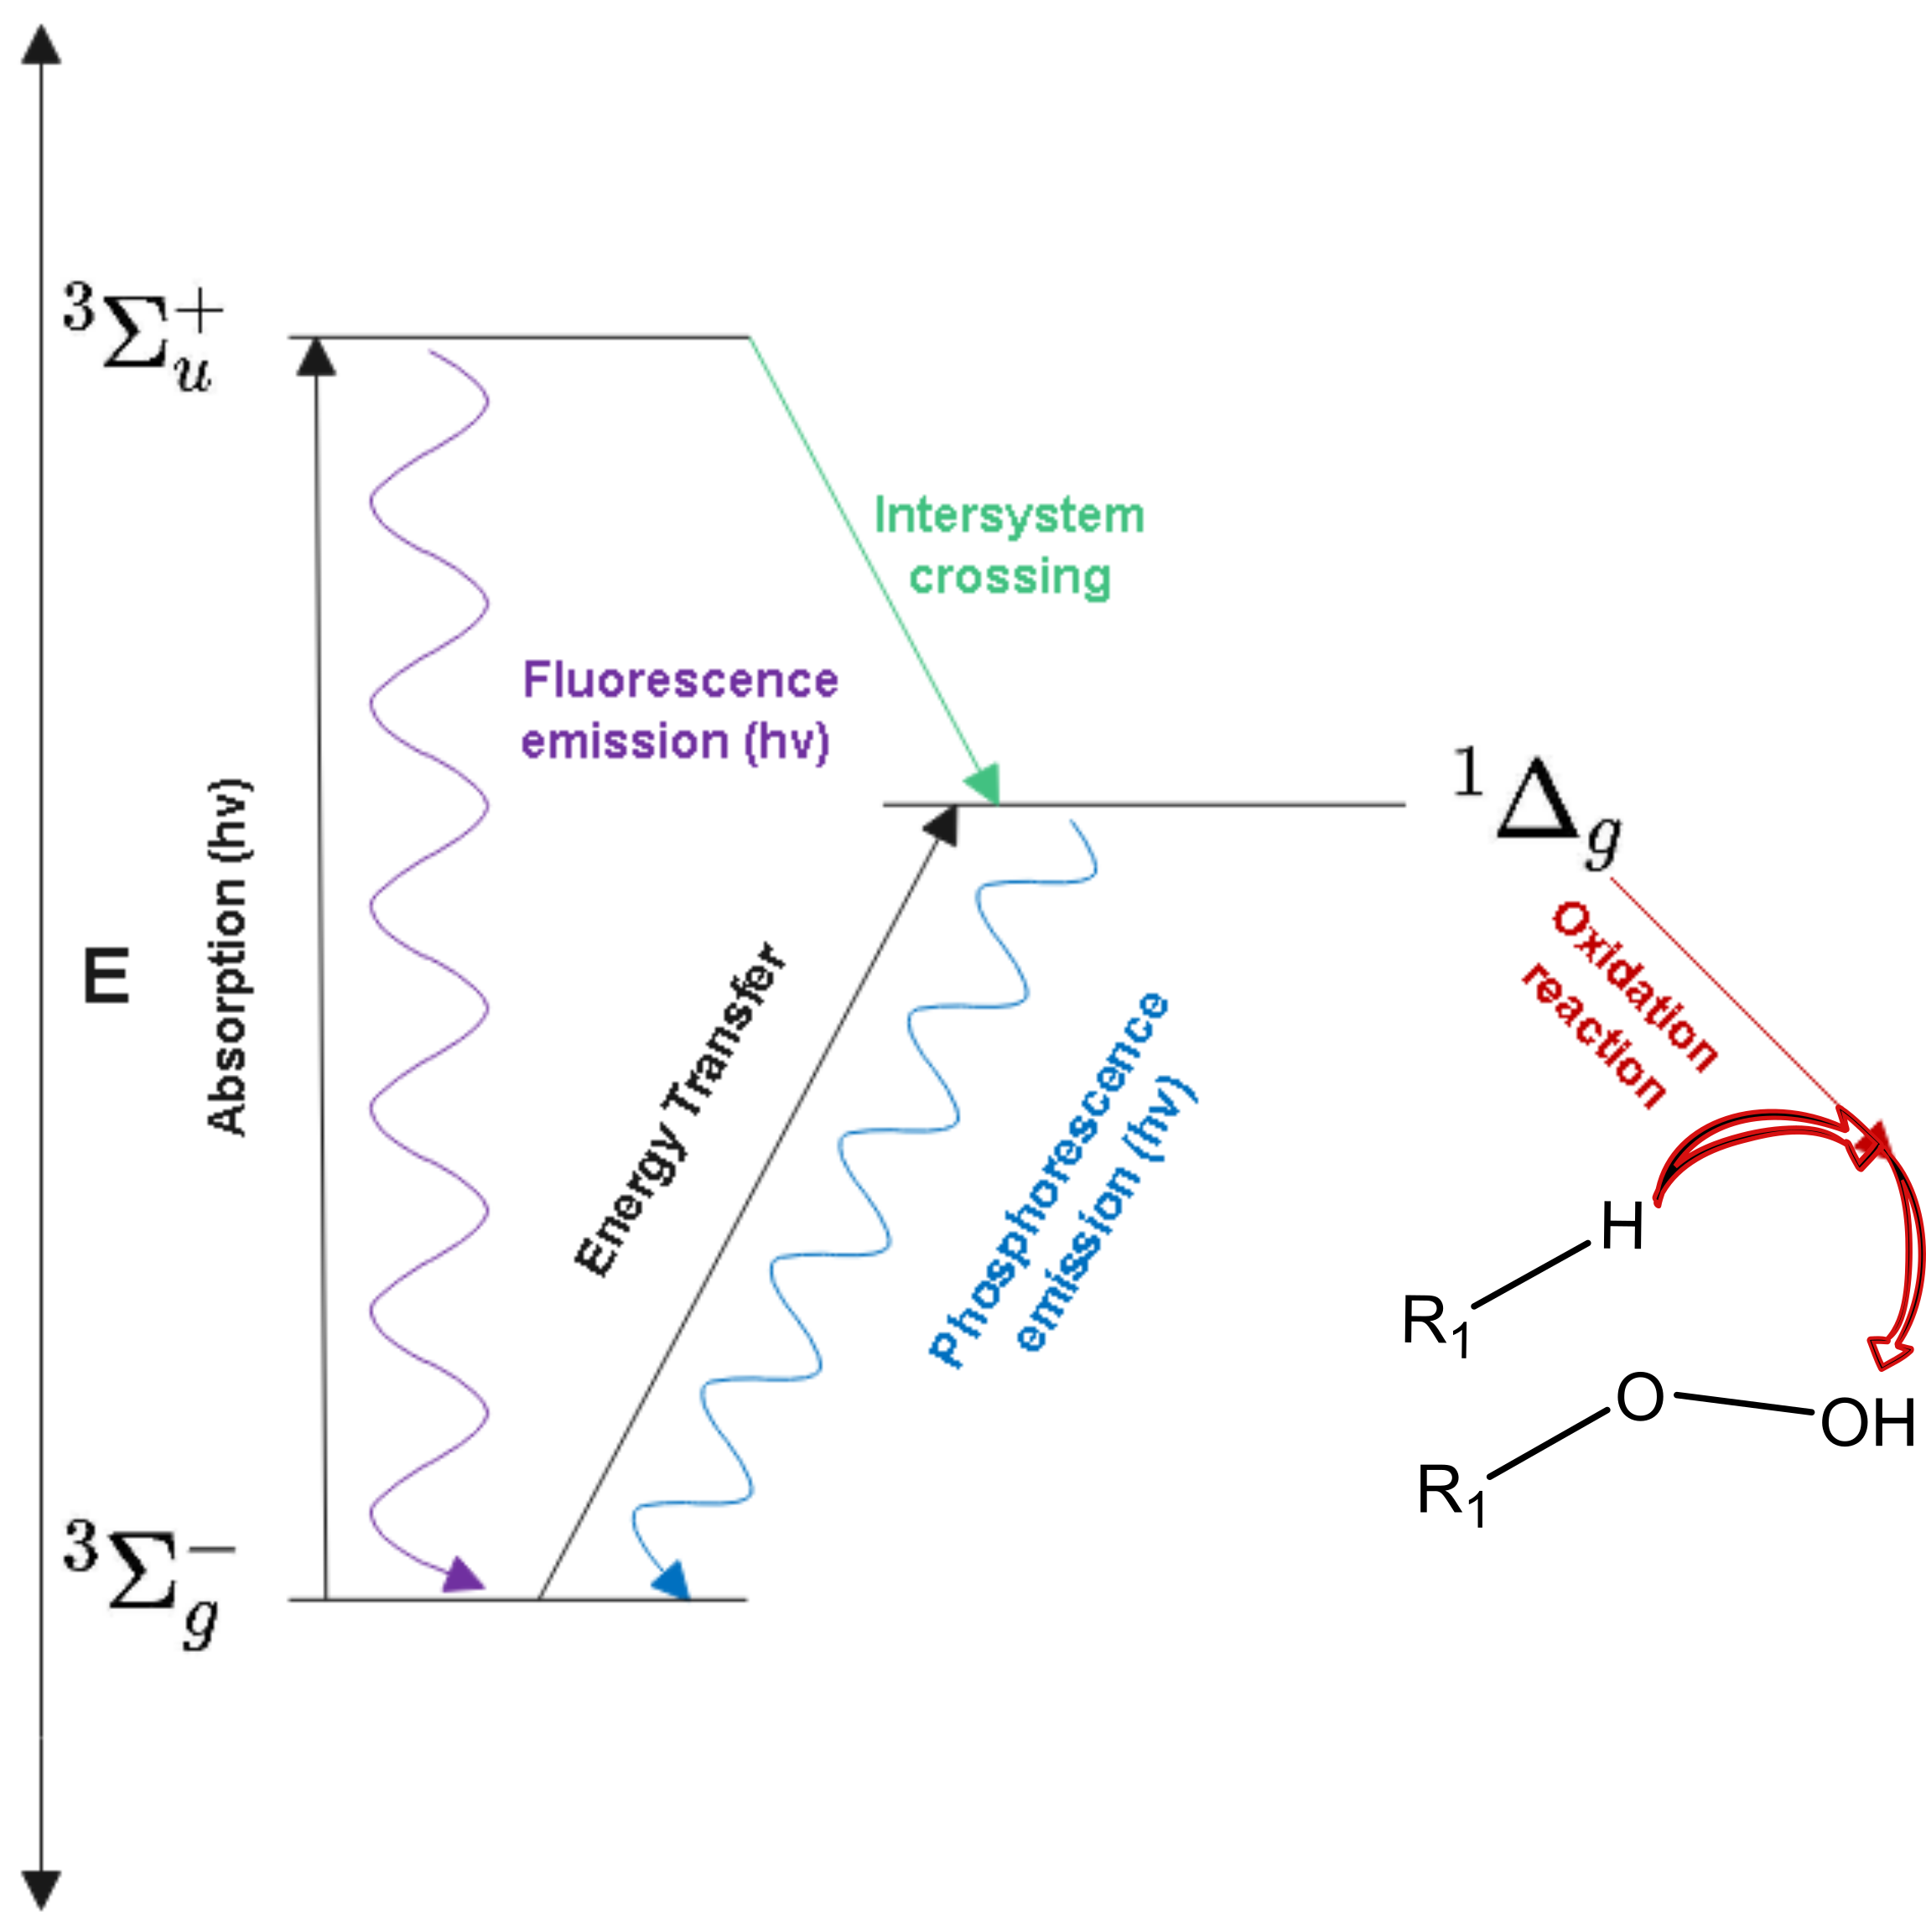
\includegraphics[width = \textwidth]{images/background/jablonski_diagram.png}
    \caption{
        A qualitative Jablonski energy diagram of photosensitization. The initial electronic absorption of a photon ($h\nu$) by $^3\Sigma_g^-$ forms a $^3\Sigma_u^+$ molecule, following the selection rules of excitation. This excited $\ce{O2}$ then either fluoresces or relaxes through intersystem-crossing into $^1\Delta_g$, which subsequently either phosphoresces or oxidizes organic substrate to form a peroxide.
    }
    \label{jablonski_diagram}
\end{figure}

\subsubsection{Photosensitizer}
The efficiency and efficacy of PDI is primarily dependent upon the chemical structure of the photosensitizer catalyst (PS), notwithstanding minor influence of the chemical conditions \cite{Kruk1998PhotophysicsLuminescence,Kullmann2012UltrafastBisporphyrin}. Two primary inefficiencies of PSs that lessen the $\Phi_{\Delta}$ are its propensities to relax through fluorescence or phosphorescence, in Figure \ref{jablonski_diagram}, and to photobleach, where irradiation and $^1\Delta_g$ irreversibly compromise molecular absorptivity \cite{Bonnett2010ChemInformTherapy,Wasser1973TheMetallochlorins}. The efficacy of PDI is influenced by the PS functionality and charge, which should 1) optimize its association with the targeted cells \cite{VanDerWal1997DeterminationBacteria,Dickson1989CellSurfaces}; 2) minimize off-target oxidation \cite{Lambrechts2005PhotodynamicMice} and host toxicities \cite{Quishida2016PhotodynamicLight} in medical applications; and 3) be amenable to permanent surface attachment in a manner that retains material properties \cite{McCoy2014PhotodynamicControl} in material applications of PDI \cite{Peddinti2018PhotodynamicThreat,Gottenbos2001AntimicrobialBacteria}. 

The cellular permeability of a PS further determines which biological entities are oxidized during PDI. Impermeable PSs generally oxidize the phospholipid fatty acids of the cytoplasmic membrane \cite{Specht1990DepolarizationAction,Ehrenberg1993ElectricAlterations} in Figure \ref{schenck_mechanism} instead of cytoplasmic contents \cite{Maisch2004AntibacterialDermatology}. This mechanism manifests in cell death through lysis \cite{Sahu2009AtomicColi,Bertoloni1987RoleCells} and generally affects gram-positive bacteria more than gram-negative bacteria \cite{Lauro2002PhotoinactivationConjugates,Merchat1996Meso-substitutedBacteria} since the latter possess a superficial lipopolysaccharide layer that protects the cytoplasmic membrane. Permeable PSs, by contrast, can penetrate a cell and thus generate $^1\Delta_g$ within the cytoplasm where cytoplasmic chemicals \cite{Bagchi1979RoleAcriflavine} such as guanine nucleotides \cite{Prat1997Determination9,Devasagayam1991FormationOxygen} are fatally oxidized. This mechanism is more effective with prokaryotes than eukaryotes \cite{Quishida2016PhotodynamicLight}, since the latter have a nuclear membrane that protects DNA, particularly guanine, from oxidation \cite{Pereira2013PhotodynamicVitro}.

A narrow range of chemicals meet these criteria of an ideal PS. Semiconductors \cite{Nelson2002PhotoconductivityDioxide,Peiro2006PhotochemicalPreparations,Linsebigler1995PhotocatalysisResults}, and some amino acid residues \cite{Lippincott-schwartz2003PhotobleachingTechniques,Jin1995PhotolysisSolution}, can electrocatalytically generate $^1\Delta_g$; however, these molecules are inefficient and/or impractical, particularly for medical applications. The most efficacious PS in nature is chlorophyll \cite{Ramel2012ChemicalPlants}, which is an organometallic porphyrinoid (Figure \ref{zinc_porphyrin}) that evolution has tuned for low rates of photobleaching and absorption of visible light -- specifically blue-violet radiation \cite{Mtangi2017ControlSplitting} via the Soret absorption band \cite{Carre1999FungicidalCerevisiae,Pereira2014InfluencePorphyrin,Ashkenazi2003PhotodynamicBacteria,Moan1986PorphyrinShGroups,Nitzan1992InactivationPorphyrins,Durantini2006PhotodynamicBacteria,Salmon-Divon2004MechanisticTetra-mesoN-methylpyridylporphine} and green-orange radiation \cite{Bertoloni2000PhotosensitizingCells} via the Q absorption band \cite{Bonnett1999PhotobleachingStudy,Jori2006PhotodynamicApplications,Gad2004TargetedMice,Zhao2019Porphyrin-basedAbsorption}. Chlorophyll, however, has not evolved traits that optimize its association with cellular targets or its compatibility with material surfaces; therefore, synthetic porphyrins \cite{Orenstein1997TheInfections,Beirao2014PhotodynamicPorphyrin,Merchat1996StudiesPorphyrins} that emulate the successful conjugated structure \cite{Huang2008Porphyrin-dithienothiopheneCells} of chlorophyll yet introduce other metal centers \cite{Mosinger1997QuantumPorphine} and functional handles  \cite{Hirao1999TheoreticalDerivatives,Wu2014BODIPY-basedSolution,Chacon1988SingletArachidonic} (e.g. Figure \ref{zinc_porphyrin}) that improve its utility in PDI \cite{Jager2016QScales,Karolczak2004PhotophysicalTetraphenylporphyrin,Mathai2007SingletTherapy} is an appealing direction for PDI research. 

\begin{figure}
    \centering
    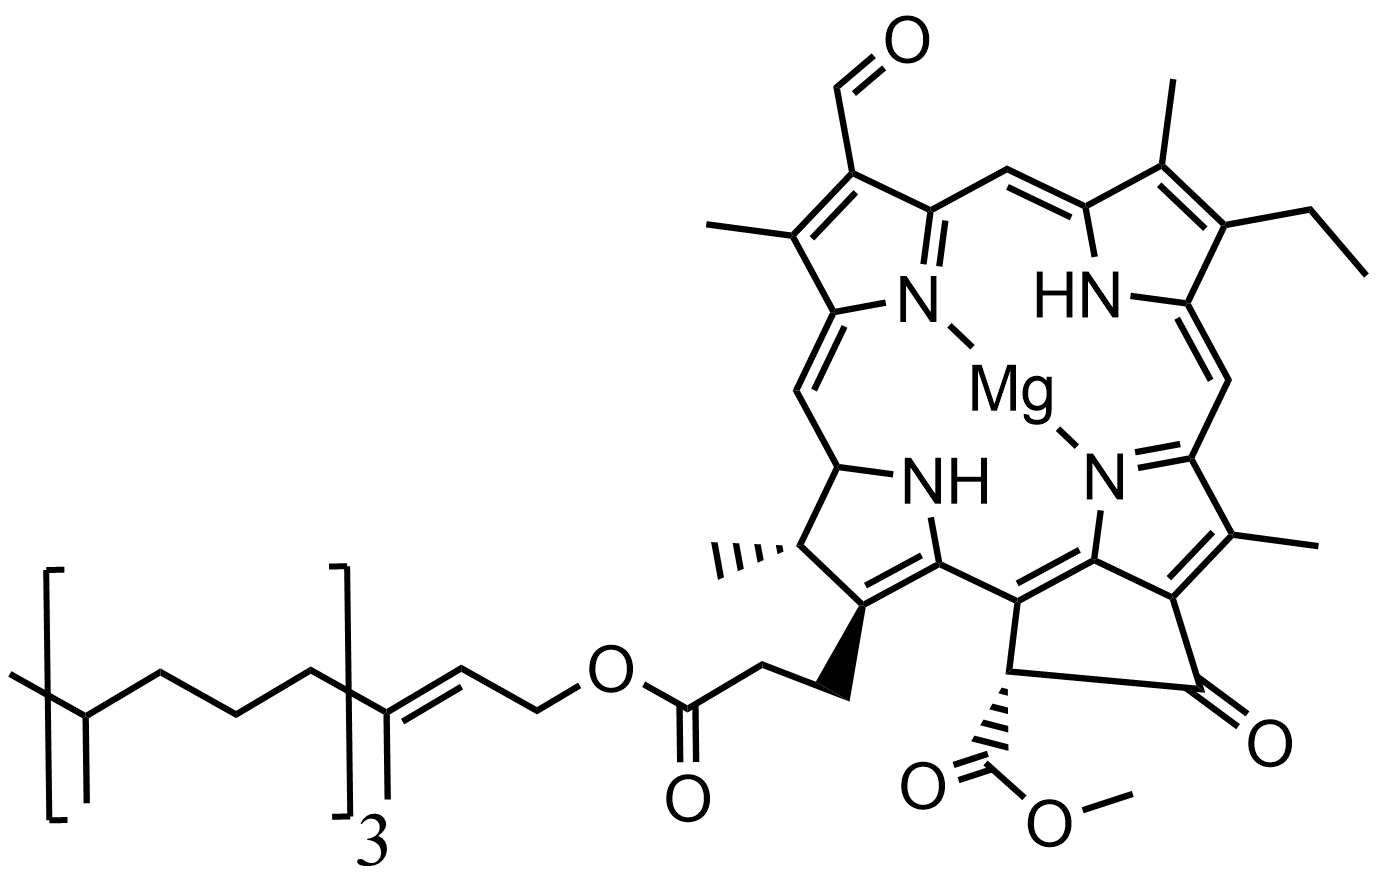
\includegraphics[width = \textwidth]{images/background/chlorophyll.png} \\
    \midrule
    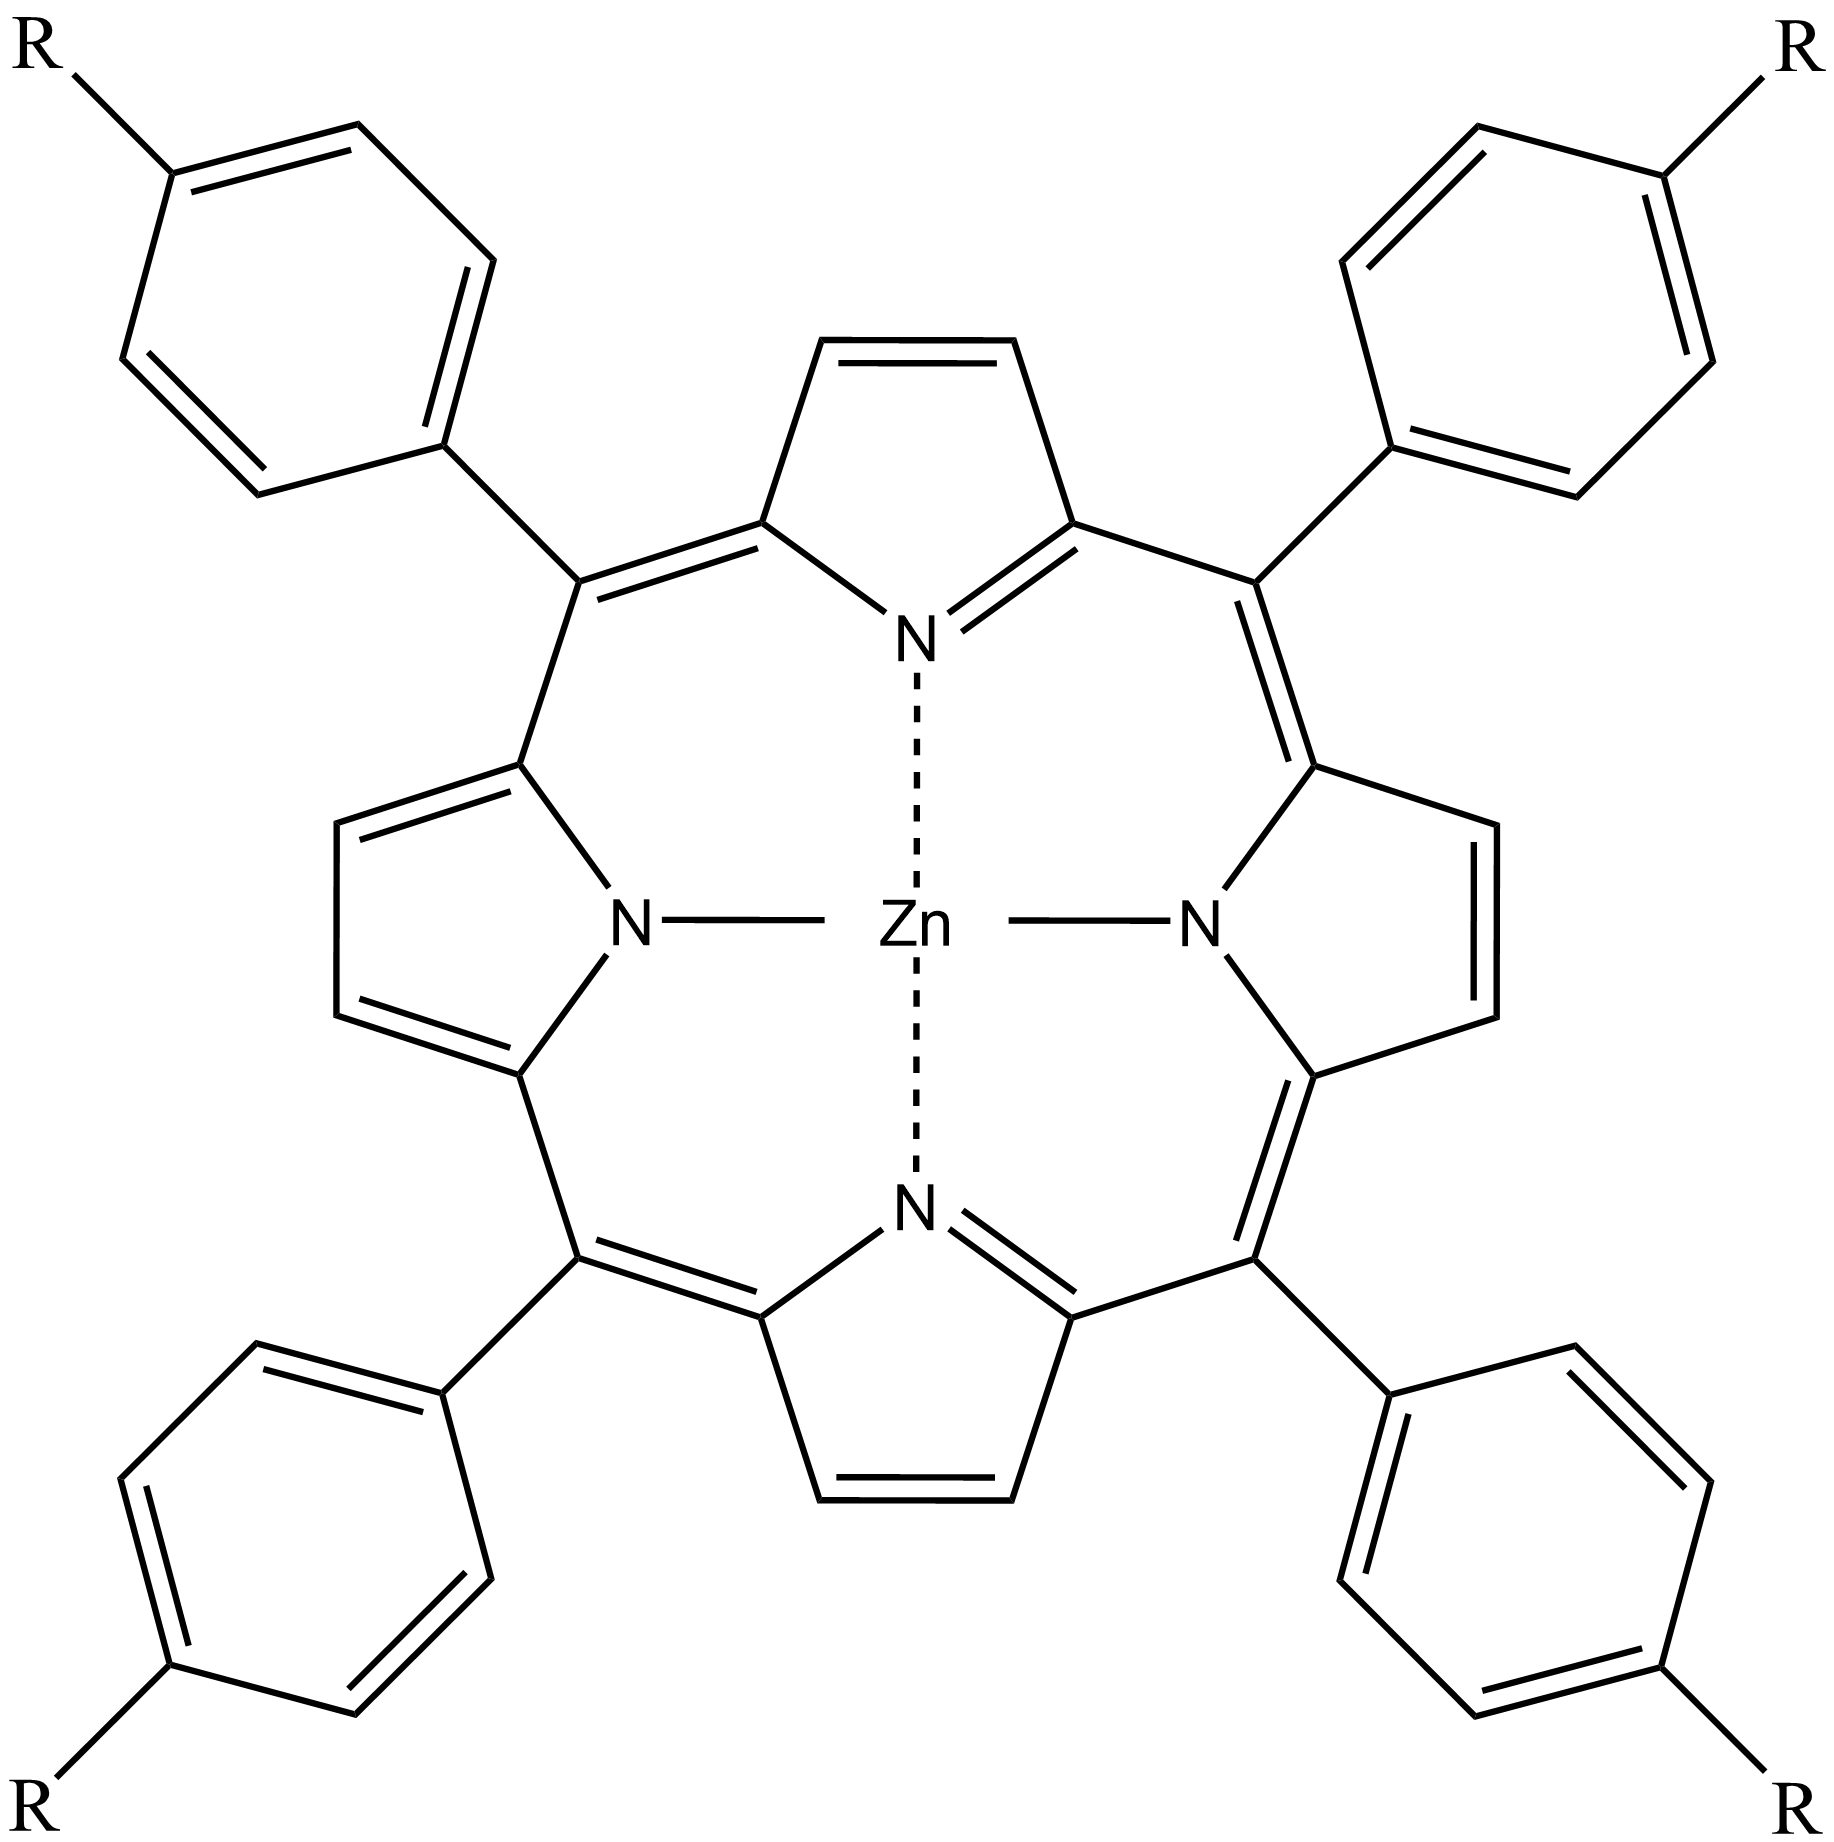
\includegraphics[width = 0.5\textwidth]{images/background/zinc_porphyrin.png}
    \caption{
        The chemical structure of porphyrinoid chlorophyll (top) juxtaposed with the core motif of a synthetic porphyrin analogue (bottom).
    }
    \label{zinc_porphyrin}
\end{figure}

\begin{figure}[t]
    \centering
    \includegraphics[width = \textwidth]{images/background/BCFA_schenck_oxidation_2.png}
    \caption{
         The reaction mechanisms of Type II oxidation and subsequent decompositions. Step (1) depicts the concerted \cite{Foote1968PhotosensitizedOxygen} Schenck reaction. Step (2) depicts the homolytic cleavage of the hydroperoxide bond to form $\ce{OH^.}$ and an oxy radical that may enter autoxidation mechanisms. Step (3) depicts radical propagation via hydrogen abstraction to form another radical substrate and an alcohol byproduct. Step (4) is a concerted Russell reaction \cite{Russell1957Deuterium-isotopeRadicals,Howard1968TheMechanism} between two peroxides that forms a $\ce{H2O2}$, an $\alpha,\beta$-ketone, and an alcohol. The reactions of Steps (2-4) sample the wide array of possible decompositions that follow oxidation mechanisms.
    }
    \label{schenck_mechanism}
\end{figure}

\subsection{PDI modeling}
Computational models of PDI that can guide experimentalists, biologists and chemists alike, through the design of more efficacious PSs and PDI systems unfortunately are scarce. Santos et al. \cite{Santos2020ApplicationAureus} developed an accurate second-order polynomial to mathematically describe the inactivation of \textit{S. aureus} as a function of time at a particular wavelength and PS concentration, however, the model is bound to a narrow range of conditions, and does not permit the investigator to explore different parameters such as PS characteristics. Brasel et al. \cite{Brasel2020AnAgalactiae} developed a sigmoidal logistic model to assess the sensitivity of PDI inactivation to incident irradiance $\frac{mW}{cm^2}$ and exposure time; however, the model likewise does not permit investigations of alternative PDI systems. Finally, Sabino et al. \cite{Sabino2019InactivationTherapy} developed a Weibull power-law function from fitted inactivation data to practically predict lethal doses and the tolerance factor of a PDI system; yet, the mathematical model is limited in scope and does not describe the fundamental chemistry of PDI. 

We therefore developed a mechanistically resolved kinetic model of PDI for an impermeable PS and encapsulated into a Python API (PDIpy) that allow investigators to efficiently explore a continuum of values for numerous parameters. The means of editing and customizing the extensive list of parameters, and understanding the default values, is detailed in the API documentation. PDIpy uses Tellurium \cite{Choi2018Tellurium:Biology} to concisely construct SBML \cite{Keating2020Models}, SED-ML \cite{Waltemath2011ReproducibleLanguage}, and COMBINE OMEX \cite{Bergmann2014COMBINEProject} descriptions of the simulations, which support transparency and reproducibility. The logistic (sigmoidal) Hill equation is then fitted to simulation predictions of cytoplasmic oxidation to systematically construct the inactivation plot based upon the oxidation predictions. We exemplify the model through replicating experimental studies and conducting a sensitivity analysis of light intensity. We expect that the open-source project will foster experimental progress in a resource efficient manner, and will inspire computational biologists to refine tools that can expedite the scientific response to the looming medical crisis of antibiotic resistance. 

\section{Methods} \label{methods}
\subsection{Conceptual model}
PDIpy conceptually represents an experimental PDI system with a coccus (spheroid) bacterium like \textit{S. aureus}. The program accepts parameters for each aspect of PDI: the light source and incident intensity; the PS absorptivity, structural dimensions, and $\frac{mol}{vol}$ or $\frac{mol}{area}$ concentration; the bacterial specie, membrane composition, and $\frac{CFU}{mL}$ for planktonic experiments; the solution dimensions; and kinetic constants for the PDI reactions. Default values for many of these parameters supplement user-defined parameters.

\subsection{Kinetic reactions}
Our model is predicated upon a set of three chemical processes that embody the essence of PDI. 1) A photoelectric interaction \cite{Wheaton2009PhotoelectricEffect} from \cref{ps_excitation_steps} occurs after $\ce{^1PS}$ is struck by a photon ($h\nu$) and undergoes intersystem crossing per to form $\ce{^3PS}$. 2) An energy transfer in \cref{excited_ps_steps} occurs from $\ce{^3PS}$ to $^3\Sigma_g^-$. 3) The $^1\Delta_g$ oxidizes biological substrates, which includes both cytoplasmic phosholipids and biofilm polymeric substances, or it irreversibly disrupts PS absorptivity through photobleaching. A complete description of this kinetic system is represented in Table \ref{reactions_table}, and each of the reactions are each detailed in the following sub-sections.

\subsubsection{User inputs}
The PDIpy API accepts a variety of parameters that allow the user to customize almost every aspect of the PDI system. These parameters are provided through either a dictionary argument in the \pyobject{define\_conditions} function, or through a JSON parameter file for each category of parameters -- e.g. light, PS, bacterium, and solution space -- that more reproducibly and transparently describes the simulated system. The complete list of accepted parameters and formats are detailed in the PDIpy documentation (\url{https://github.com/freiburgermsu/PDIpy/blob/main/README.rst}).

\begin{table}[]
    \centering
    \begin{tabular}{c|c}
        \textbf{Name} & \textbf{Reaction} \\
        \toprule
        Photoexcitation & \ce{^1PS <=> ^3PS} \\
        Photobleaching & \ce{^1PS + ^1\Sigma_g -> ^1PS_{bleached}} \\
        Energy transfer & \ce{^3PS + ^3\Sigma_g^- -> ^1PS + ^1\Delta_g} \\
        Phosphorescence & \ce{^1\Delta_g -> ^3\Sigma_g^-} \\
        Membrane oxidation & \ce{^1\Delta_g + FA -> FA-OOH} \\
        EPS oxidation & \ce{^1\Delta_g + EPS -> EPS-OOH} \\
    \end{tabular}
    \caption{
        Each chemical reaction of the PDI kinetic model is presented. These reactions are individually detailed in section \ref{methods}.
    }
    \label{reactions_table}
\end{table}

\subsubsection{Photoelectric}
\paragraph{PS excitation}
PDI begins with the excitation of the PS. This occurs as the combined result of an incident photon i) entering the aqueous solution, ii) striking a PS, and then iii) exciting an electron of a PS. This sequence is encapsulated in the kinetic expression
\begin{multline} \label{ps_excitation_kinetics}
    \frac{d[\ce{^3PS}]}{dt} =  k_{excitation}*\frac{photons_{PS}}{photons_{total}} \\ 
    *\Phi_{excitation}*[\ce{^1PS}] - k_{fluorescence}*[\ce{^3PS}]~. 
\end{multline}
The $k_{excitation}$ \& $k_{fluorescence}$ rate constants are estimated as the inverse of the rise and decay times for the selected PS, respectively. The approximate rise time for a porphyrin PS is $50 fs$, which is consistent with estimates of $<100 fs$ \cite{Andersson1999PhotoinducedState} and $60-90 fs$ in ethanol solvent \cite{Gurzadyan1998Time-resolvedZn-tetraphenylporphyrin} which elongates the lifetime of excited molecules relative to water. The decay time, as the S2 fluorescence \cite{Akimoto1999UltrafastPorphyrins}, and $\Phi_{excitation}$ ($\frac{PS excited}{photon absorbed}$) are approximated for a porphyrin PS as $1.5 ns$ and $\approx 0.7$ \cite{Krasnovsky2012PhotochemicalEnvironment}, respectively. The $\frac{photons_{PS}}{photons_{total}}$ \cite{Brasel2020AnAgalactiae}, which is the proportion of photons in the solution that strike a photosensitizer \cite{Santos2020ApplicationAureus}. This can be either measured as an absorbance at each wavelength \cite{Gerola2012ChemicalPhotobleaching} or calculated from the following series of steps and approximations. 1) The reported intensity of incident light from the respective light source -- i.e. irradiance ($\frac{mW}{cm^2}$), lux ($\frac{lumen}{m^2}$), or lumens (lumens) -- is converted into $watts_{incident}$ ($\frac{J}{s}$). 2) This incident wattage is attenuated by the proportion of the emission spectrum $light_{incident}$ that resides within the excitation spectrum of the parameterized PS $light_{excitation}$, 
\begin{equation}
    watt_{excitation} = \frac{light_{excitation}}{light_{incident}}*watts_{incident}.
\end{equation}
3) The $watt_{excitation}$ is then used to calculate the moles of incident photons that strike photosensitizers per timestep 
\begin{multline} \label{photons_per_second}
    \frac{photons_{PS}}{timestep}=\frac{<h\nu_{excitation}>}{h*c}*watts_{excitation} \\
    *\frac{second}{timestep}*reflection*scattering*\frac{1 mole}{N_A}*\frac{vol_{PS}}{vol_{total}},
\end{multline}
where $reflection \approx 96 \%$ and represents the proportion of incident photons that penetrate an aqueous solution \cite{Gross1993SingletLiposomes}; and $scattering$  
\begin{equation}
    \frac{I_z}{I_0} = e^{-k*z}~,
\end{equation}
represents the proportion of light $\frac{I_z}{I_0}$ that reaches a specified depth $z$ \cite{RobertW.1973TheSea}, where $k$ is the attenuation coefficient that is $\approx 0.04~(\frac{1}{m})$ \cite{Lorenzen1972ExtinctionPhytoplankton} for clear water. The $\frac{vol_{PS}}{vol_{total}}$ represents the volume proportion of the PS ($vol_{PS}$) -- calculated as the product of the quantity of PS molecules and the volume per molecule per its structure -- to the total volume of the solution in which the PS resides ($vol_{total}$). The average excitation wavelength of the PS ($<h\nu_{excitation}>$) is calculated as the weighted average of the Soret and Q excitation bands, in proportion to their relative contribution in generating $^1\Delta_g$ \cite{Nitzan2001PhotoinactivationWavelengths,Hoenes2020PhotoinactivationWavelength}, since this averaged wavelength simultaneously embodies contributions of both excitation bands. The resultant $\frac{photons_{PS}}{timestep}$ from \cref{photons_per_second} is then divided by the $\frac{photons_{total}}{timestep}$ to complete the kinetic expression in \cref{ps_excitation_kinetics} that calculates the excitation of PS in each timestep. 

\paragraph{Photobleaching}
The collision of a PS and a photon, instead of resulting in excitation, may disrupt the conjugated PS system and prevent further excitation. The reaction may be either oxygen independent, first-order, reaction \cite{Bonnett1999PhotobleachingStudy,Mang1987PhotobleachingTherapy} or a oxygen dependent, second-order, reaction 
\begin{equation}
    \ce{^3PS + ^1\Delta_g ->[h\nu] PS-OOH}~.
\end{equation}
The second-order reaction is purported to be more consequential in measured systems, thus, we implemented its kinetic expression 
\begin{equation} \label{bleaching_kinetics}
    \frac{d[\ce{^1PS_{bleached}}]}{dt} = k_{bleaching}*[\ce{^1PS}]*[^1\Delta_g]~,
\end{equation}
where the $k_{bleaching}$ rate constant $\approx 600 \frac{cm^2}{J*M}$ \cite{Dysart2005CalculationCells} for porphyrins and is a function of light exposure $\frac{J}{cm^2}$.

\subsubsection{Energy Transfer}
The energy transfer from $\ce{^3PS}$ to $^3\Sigma_g^-$  in \cref{excited_ps_steps} is described with by the kinetics expression
\begin{equation} \label{energy_transfer_kinetics}
    \frac{d[^1\Delta_g]}{dt} = k_{transfer}*\Phi_{transfer}*[^3PS]*[^3\Sigma_g^-]. 
\end{equation}
The rate constant $k_{transfer}$ is the inverse of the decay time of $\ce{^3PS}$, which for a porphyrin PS appears to be $100 ns$ in aqueous after accounting for the reported value \cite{Kupper2002KineticsOxygen} in acetone solvent that significantly increases the lifetime of excited states \cite{Spikes1992QuantumUroporphyrin}. The $^1\Delta_g$ phosphorescence side reaction, which often emits a specific infrared wavelength that can be measured to approximate the $[^1\Delta_g]$ \cite{Macpherson1993DirectCentres}, is kinetically represented 
\begin{equation}
    \frac{d[^3\Sigma_g^-]}{dt} = k_{phosphorescence}*[^1\Delta_g]
\end{equation}
where $k_{phosphorescence}$ is a function of $\frac{CFU}{mL}$, since the $^1\Delta_g$ lifetime is greater in biological material and thus it is proportional with the bacterial concentration in planktonic simulations \cite{Maisch2007TheBacteria}. The minimum lifetime is limited to $3.5\mu s$ for pure water \cite{Baier2005Time-resolvedCells}.

\subsubsection{Oxidation}
The oxidation reactions are the primary consumers of oxygen in the kinetic system. The simulated system, however, is assumed to possess an equilibrium between the solution and the atmosphere, which prevents the depletion of oxygen in the system. This is represented by replacing each oxygen molecule that is consumed during the oxidation of biological substrate in \cref{membrane_oxidation,EPS_oxidation}.

\paragraph{Cytoplasmic membrane} 
The oxidation of cytoplasmic phospholipids, which we approximate as fatty acid chains, is represented as an irreversible second-order reaction \cite{Watabe2007OxidationMembranes.}
\begin{equation} \label{membrane_oxidation}
    \ce{^1\Delta_g + FA -> FA-OOH}.
\end{equation}
and a second-order kinetic expression
\begin{equation} \label{membrane_oxidation_kinetics}
    \frac{d[FA-OOH]}{dt} = k_{fa}*[^1\Delta_g]*[FA]~.
\end{equation}
The rate constant $k_{fa} \approx 769 \frac{L}{g*s}$ \cite{Mukai2019KineticSolution} and the concentration of fatty acid chains in the cytoplasmic membrane is described in units of $\frac{g}{L}$, after calculating the weighted average MW of fatty acids within the membrane. 

\paragraph{Biofilm matrix} 
The oxidation of EPS is reported to be significant during PDI \cite{Beirao2014PhotodynamicPorphyrin}. This process is represented through an irreversible reaction
\begin{equation} \label{EPS_oxidation}
    \ce{^1\Delta_g + EPS -> EPS-OOH},
\end{equation}
which competes with \cref{membrane_oxidation} for $^1\Delta_g$ and thereby lessens the efficacy of PDI upon biofilms relative to planktonic organisms. The oxidation of bioiflm polymers is kinetically represented  
\begin{equation} \label{EPS_oxidation_kinetics}
    \frac{d[EPS-OOH]}{dt} = k_{EPS_{oxidation}}*[^1\Delta_g]
\end{equation}
with an empirical rate constant that we approximated as $37.75~\frac{1}{s}$ for \textit{S. aureus}, and an initial concentration of EPS that is $9x$ greater than the cellular mass, in proportion to mass distributions of biofilms \cite{Flemming2010TheMatrix}.

\subsection{Inactivation fitting}

Simulation results of chemical concentrations over time are processed into predictions of bacterial inactivation through a series of mathematical steps. 1) The proportion of oxidized substrate
\begin{equation} \label{oxidation_proportion}
    ox_{proportion} = \frac{[FA-OOH]}{[FA-OOH]+[FA]}
\end{equation}
is fitted to a sigmoidal curve, similar to other models \cite{Xiong1999AInactivation}. We used the Hill-equation \cite{Gesztelyi2012ThePharmacology} as a sigmoidal model of biochemistry that derives from mass-action kinetics similar to the Michaelis-Menten kinetic model. A fitting module for the Hill-equation did not exist prior to our work; hence, the HillFit Python module was developed to fit the oxidation predictions with a variation of the Hill-equation \cite{Inoue2016OscillationActivation} 
\begin{equation} \label{hill_eq}
    y=bottom+\frac{(top-bottom)*x^n}{EC50^n+x^n}
\end{equation}
that improves its fit to data. The regression parameters from the fitted Hill equation are then systematically adjusted to construct an inactivation plot that replicates experimental results while preserving the underlying Hill-equation relationship. These parameter adjustments are presented in Table \ref{hill_parameters} for both simulations of planktonic and biofilm bacteria. The top parameter of \cref{hill_eq} is adjusted asymptotically to a limit that follows an subtly different empirical expression for planktonic $1-10^{-\Omega}$ than biofilm $1-10^{-0.7-\Omega }$ simulations, where $\Omega = wattage^{\frac{1}{5}}-log10(1-final_{oxidation\_proportion})$. This top limit is empirically determined to manifest in the log-inactivation predictions being 1-2 greater than the log-oxidation from \cref{oxidation_proportion}, which embodies our assumption -- implicit in experimental studies -- that $1-10\%$ of membrane phospholipids must oxidize for a cell to lyse. The different parameter adjustments for sessile versus planktonic bacterial systems is that biofilms possess numerous factors, such as heterogeneous diffusion rates, that are not explicitly considered in our kinetic model, and thus custom equation adjustments are our means of compensating these factors into the final predictions. 

\begin{table}[]
    \centering
    \begin{tabular}{l|c|c}
        \textbf{Bacterial state} & \textbf{Hill parameter} & \textbf{Adjustment} \\
        \multirow{2}{}{Planktonic} & EC50 & -76\% \\
         & nH & +100\% \\
         \midrule
         \multirow{2}{}{Biofilm} & EC50 & -65\% \\
         & nH & +120\% \\
    \end{tabular}
    \caption{
        The Hill parameters adjustments that are enacted to create the inactivation plot for both planktonic and biofilm systems. 
    }
    \label{hill_parameters}
\end{table}

% \subsubsection{Cross-linked systems}

% \paragraph{iPDIpy}
% The PDIpy API is graphically interactive through a user interface iPDIpy, which is depicted in Figure \ref{}. This interface provides a convenient means for parameterizing a PDIpy simulation, exporting and importing sets of parameters, parsing the processed simulation data, viewing error messages and calculated values, viewing the output figure of bacterial reduction over time, and parsing the processed data through a build-in function. The iPDIpy version of PDIpy is downloadable from our GitHub repository.

% \begin{figure}
%     \centering
%     \includegraphics{}
%     \caption{
%         The left pane of the GUI will contain command buttons like restarting the simulation or export results, while the right pane will edit the simulation data and or bacterial qualities/species.
%     }
%     \label{iPDIpy_interface}
% \end{figure}


\section{Case Studies}
A PDI experiment from literature that thoroughly described its experimental procedure was parameterized into PDIpy, and the resultant predictions were compared with the reported results. These comparisons all pertain to \textit{S. aureus}, which is a model coccus bacterium that is abundantly studied with PDI and AMR infections as MRSA.

% \subsection{Cross-linked PS}
% Experimental data from our lab with cross-linked PSs (unpublished) was parameterized, in Table \ref{}, into PDIpy. The predicted reduction curve over time in Figure \ref{} agreed with the experimental data at the measured time of 6 hours and 98\% reduction, which supports that the software yields accurate predictions. 

% \paragraph{}
% .

% \subsection{Solution PS}

\paragraph{Beirao et al.\cite{Beirao2014PhotodynamicPorphyrin}}
This paper experimentally examines the efficacy of a dissolved PS, over a range of concentrations, against both planktonic and sessile bacterial states. The ample details of experimental conditions were parameterized into PDIpy, and the predicted log-inactivation was contrasted with the reported log-inactivation at various times, concentrations, and bacterial states in Table \ref{beirao_et_al_data}. The predicted log-oxidation and log-inactivation for a few of the simulated conditions are plotted in Figure \ref{beirao_et_al}. These plots cannot be contrasted with reported data since log-inactivation was only reported by Beirao et al. at one time, and not over a continuum of times that would be required to populate a figure. The regression plots from fitting the Hill-equation to the log-oxidation results of Figure \ref{beirao_et_al} is depicted in Figure \ref{hill_regression}, respectively, where the very precise fitting -- $R^2 > 0.996$ -- supports that our kinetic model of PDI fundamentally recreates the biochemical relationship that is predicted by the Hill model of kinetics.

\begin{table}[h]
    \centering
    \begin{tabular}{c|c|c|c|c|c}
        Bacterial & [PS] & Inactivation & Reported & Predicted & \multirow{2}{1.2cm}{\%-error}\\
        state & ($\mu m$) & (-log10) & (min) & (min) & \\
        \toprule
        \multirow{3}{1.5cm}{planktonic} & 5 & 7.6 & 51 & 117 & 119\\
        & 10 & 7.6 & 51 & 36 & -29\\
        & 20 & 7.6 & 42 & 12 & -71\\
        \midrule
        \multirow{3}{1.5cm}{sessile} & 5 & 3.6 & 390 & 566 & 45\\
        & 10 & 5 & 390 & 310 & -20\\
        & 20 & 6.3 & 390 & 247 & -37\\
        \bottomrule
    \end{tabular}
    \caption{
        A quantitative comparison of inactivation data from Beirao et al. versus PDIpy predictions. 
    }
    \label{beirao_et_al_data}
\end{table}

\begin{figure}
    \centering
    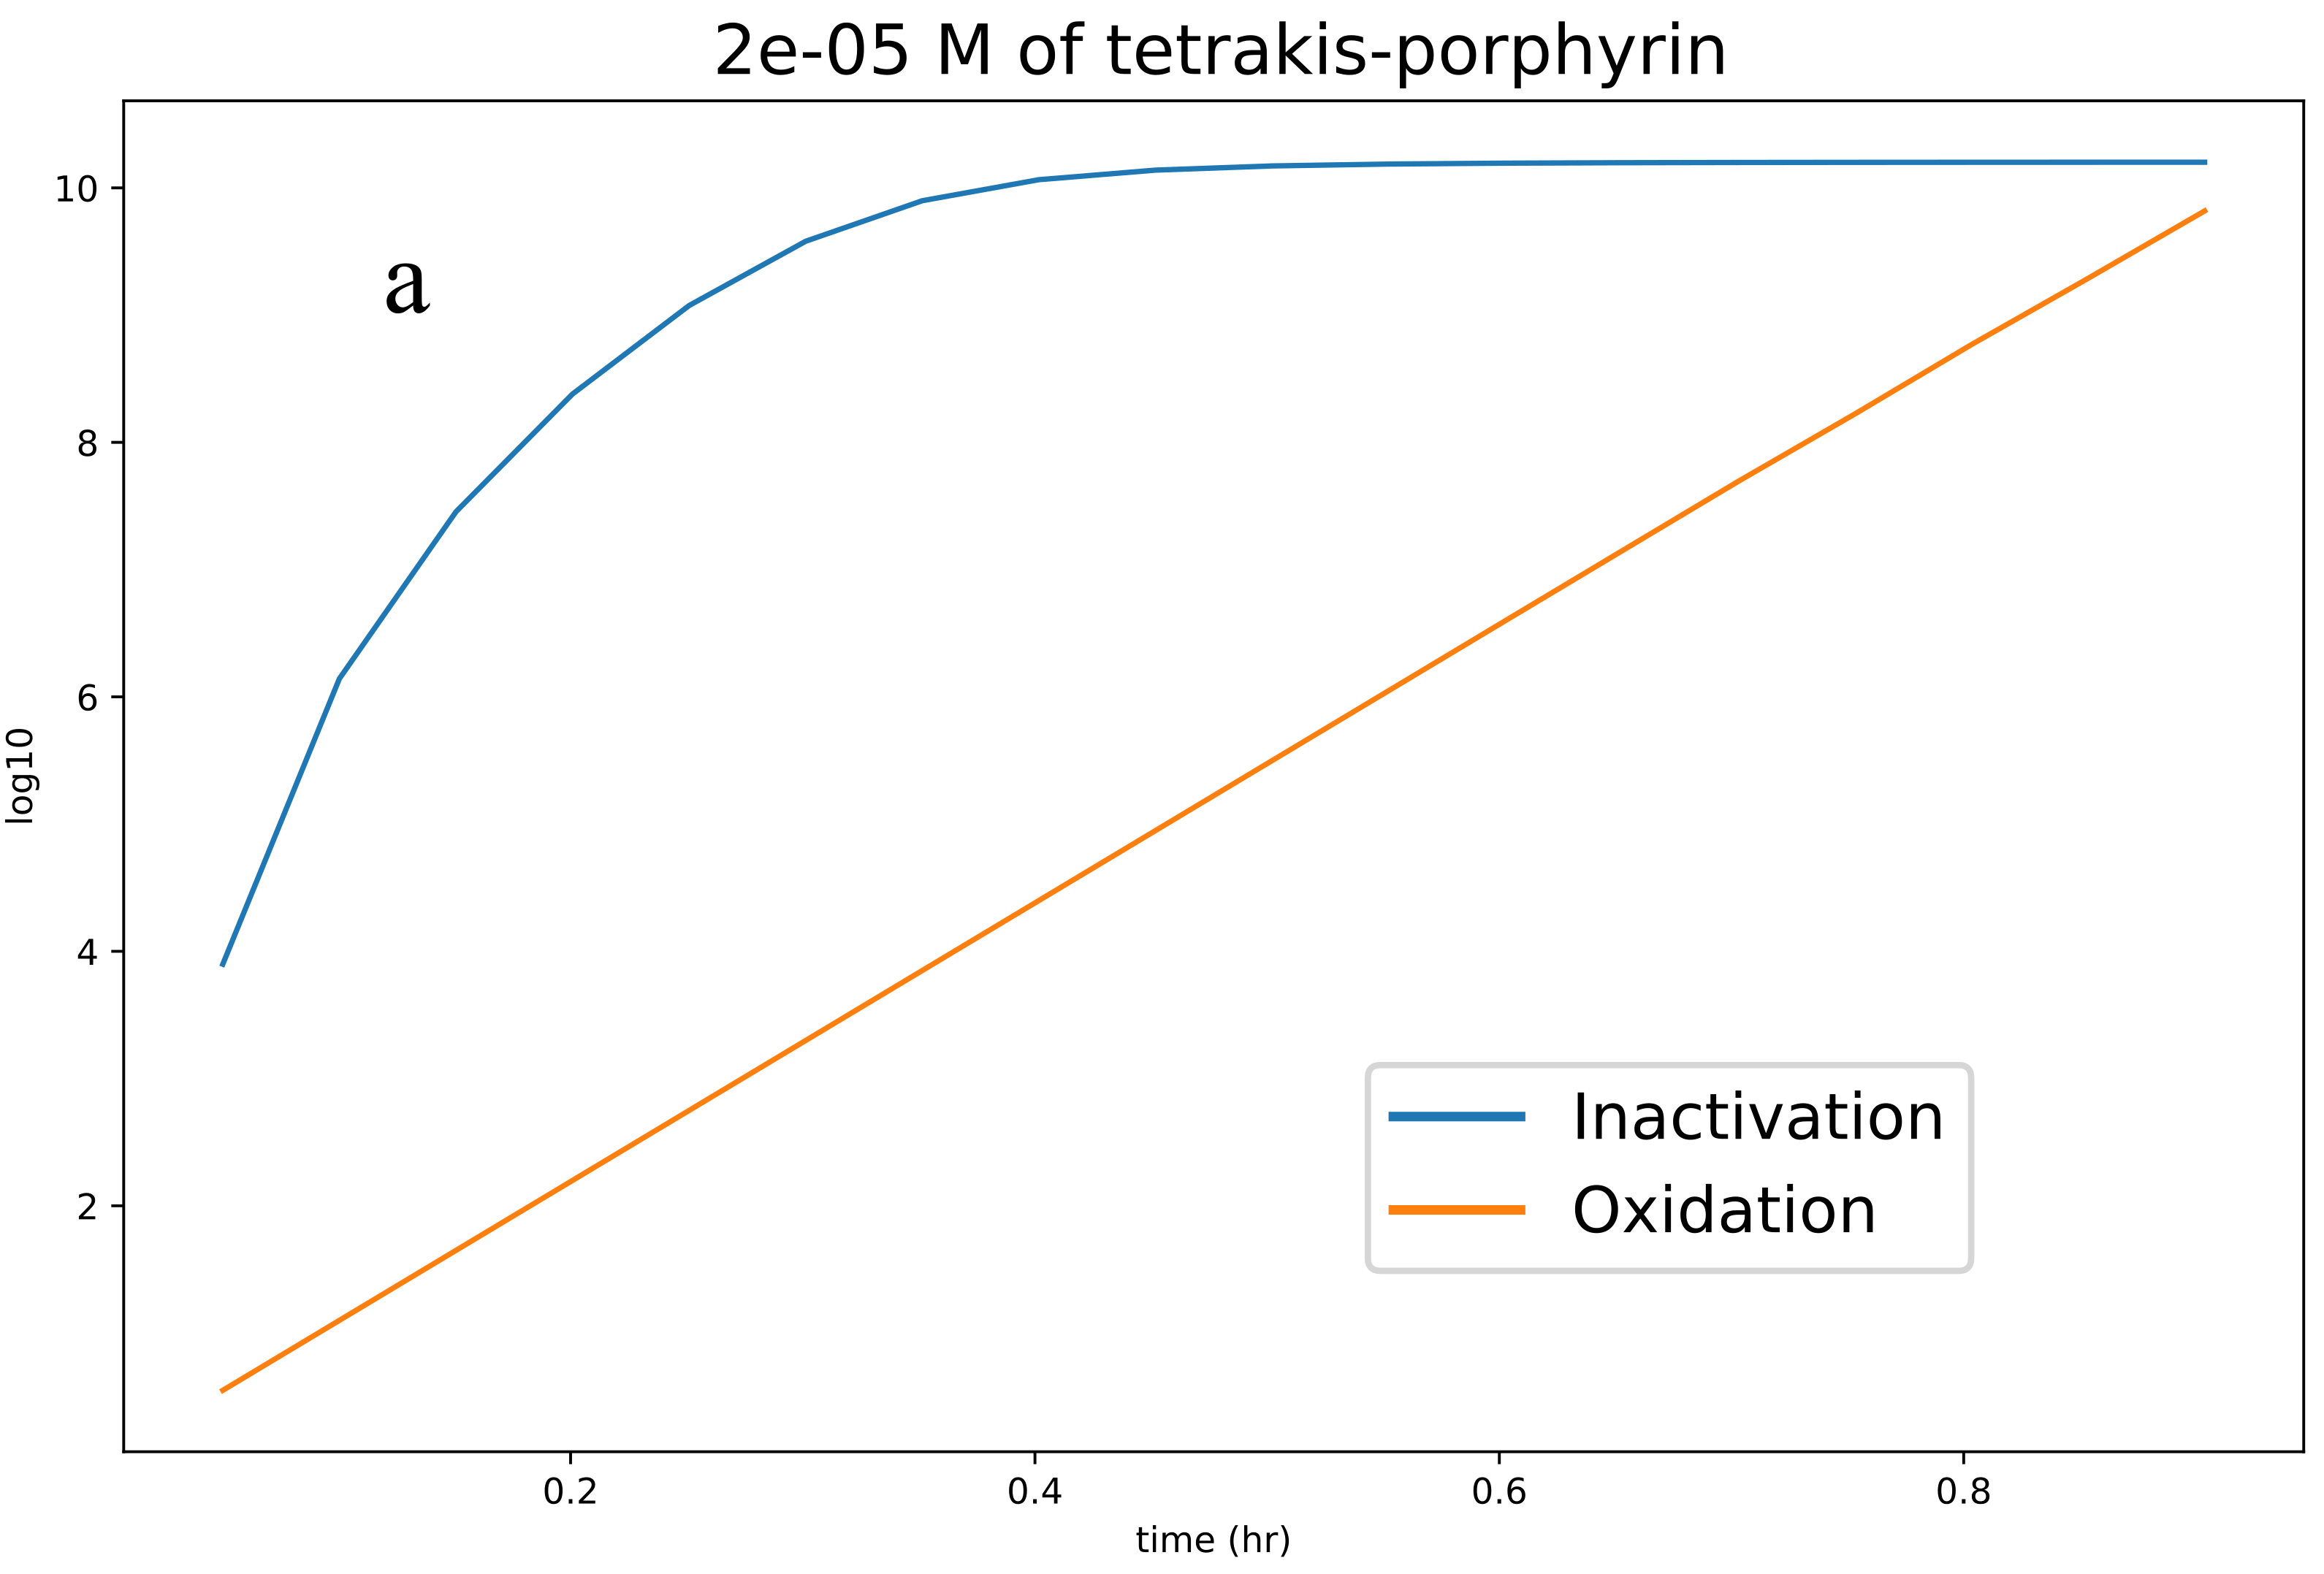
\includegraphics[width = 0.9\textwidth]{images/examples/20uM.png}
    \vspace{5mm}
    \midrule
    \vspace{5mm}
    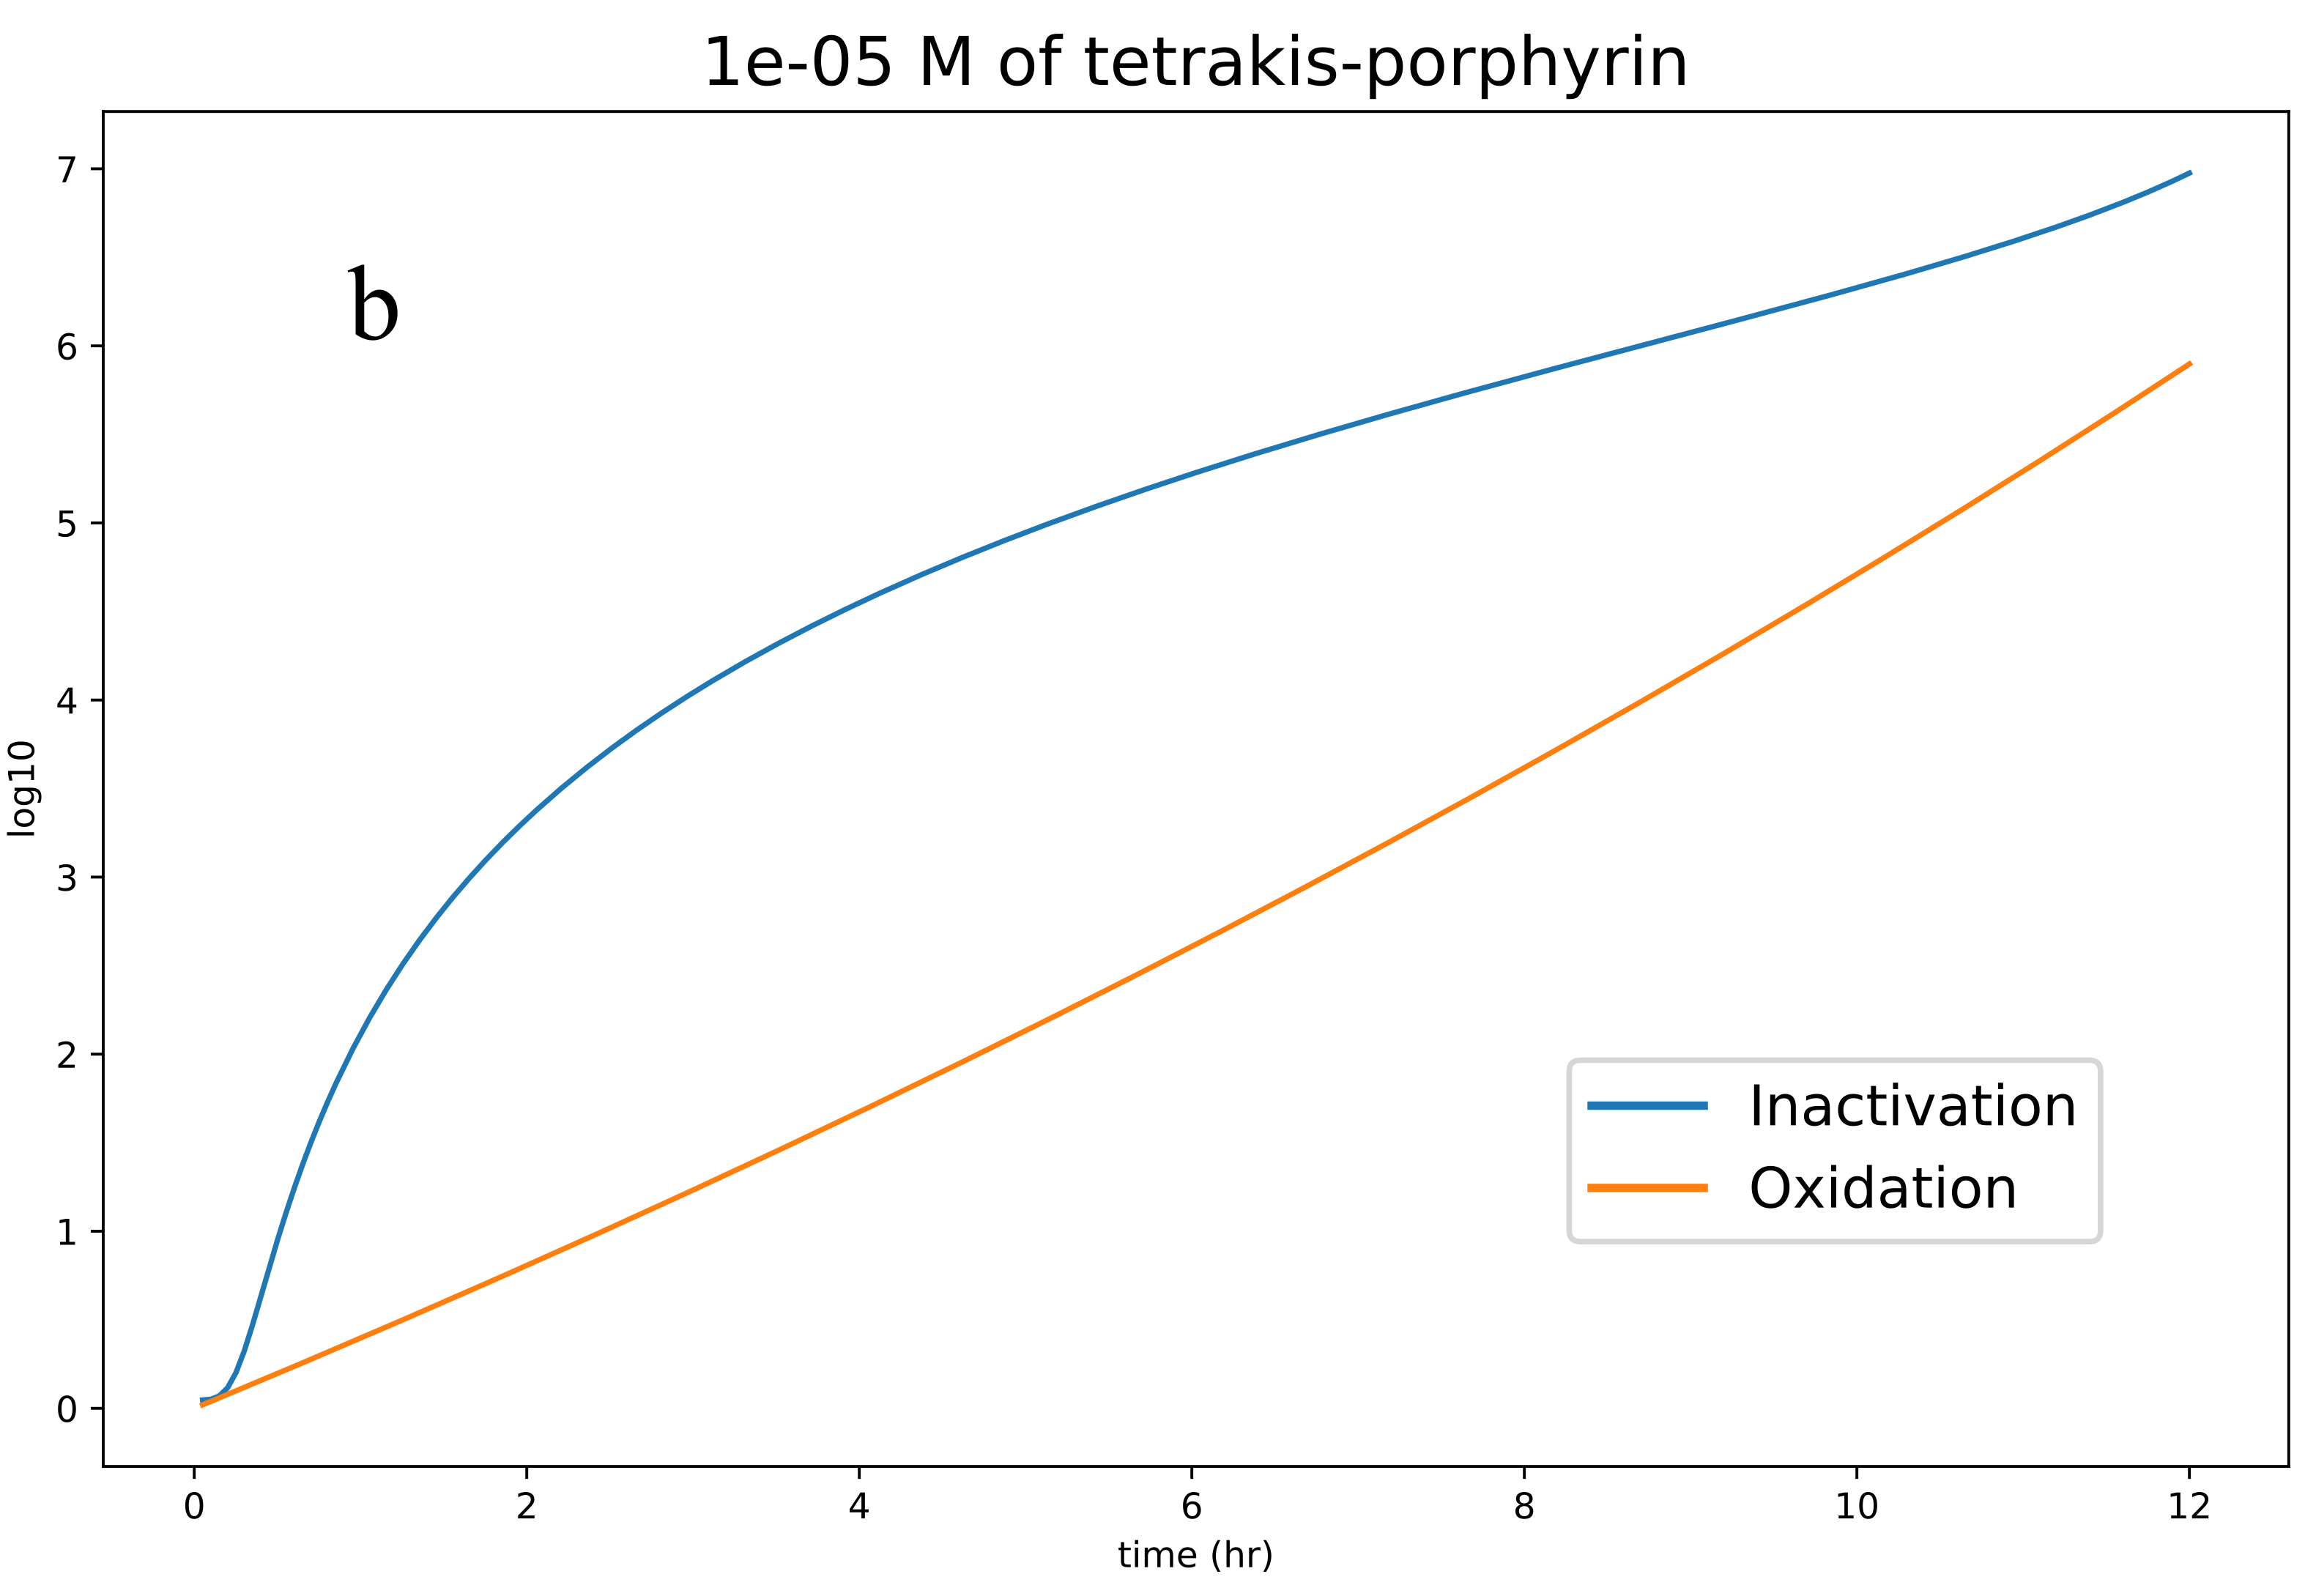
\includegraphics[width = 0.9\textwidth]{images/examples/10uM_biofilm.png}
    \caption{
        Two exemplary figures of PDIpy replications of the Beirao et al. data for a) planktonic and b) biofilm bacterial states.
    }
    \label{beirao_et_al}
\end{figure}

\begin{figure}
    \centering
    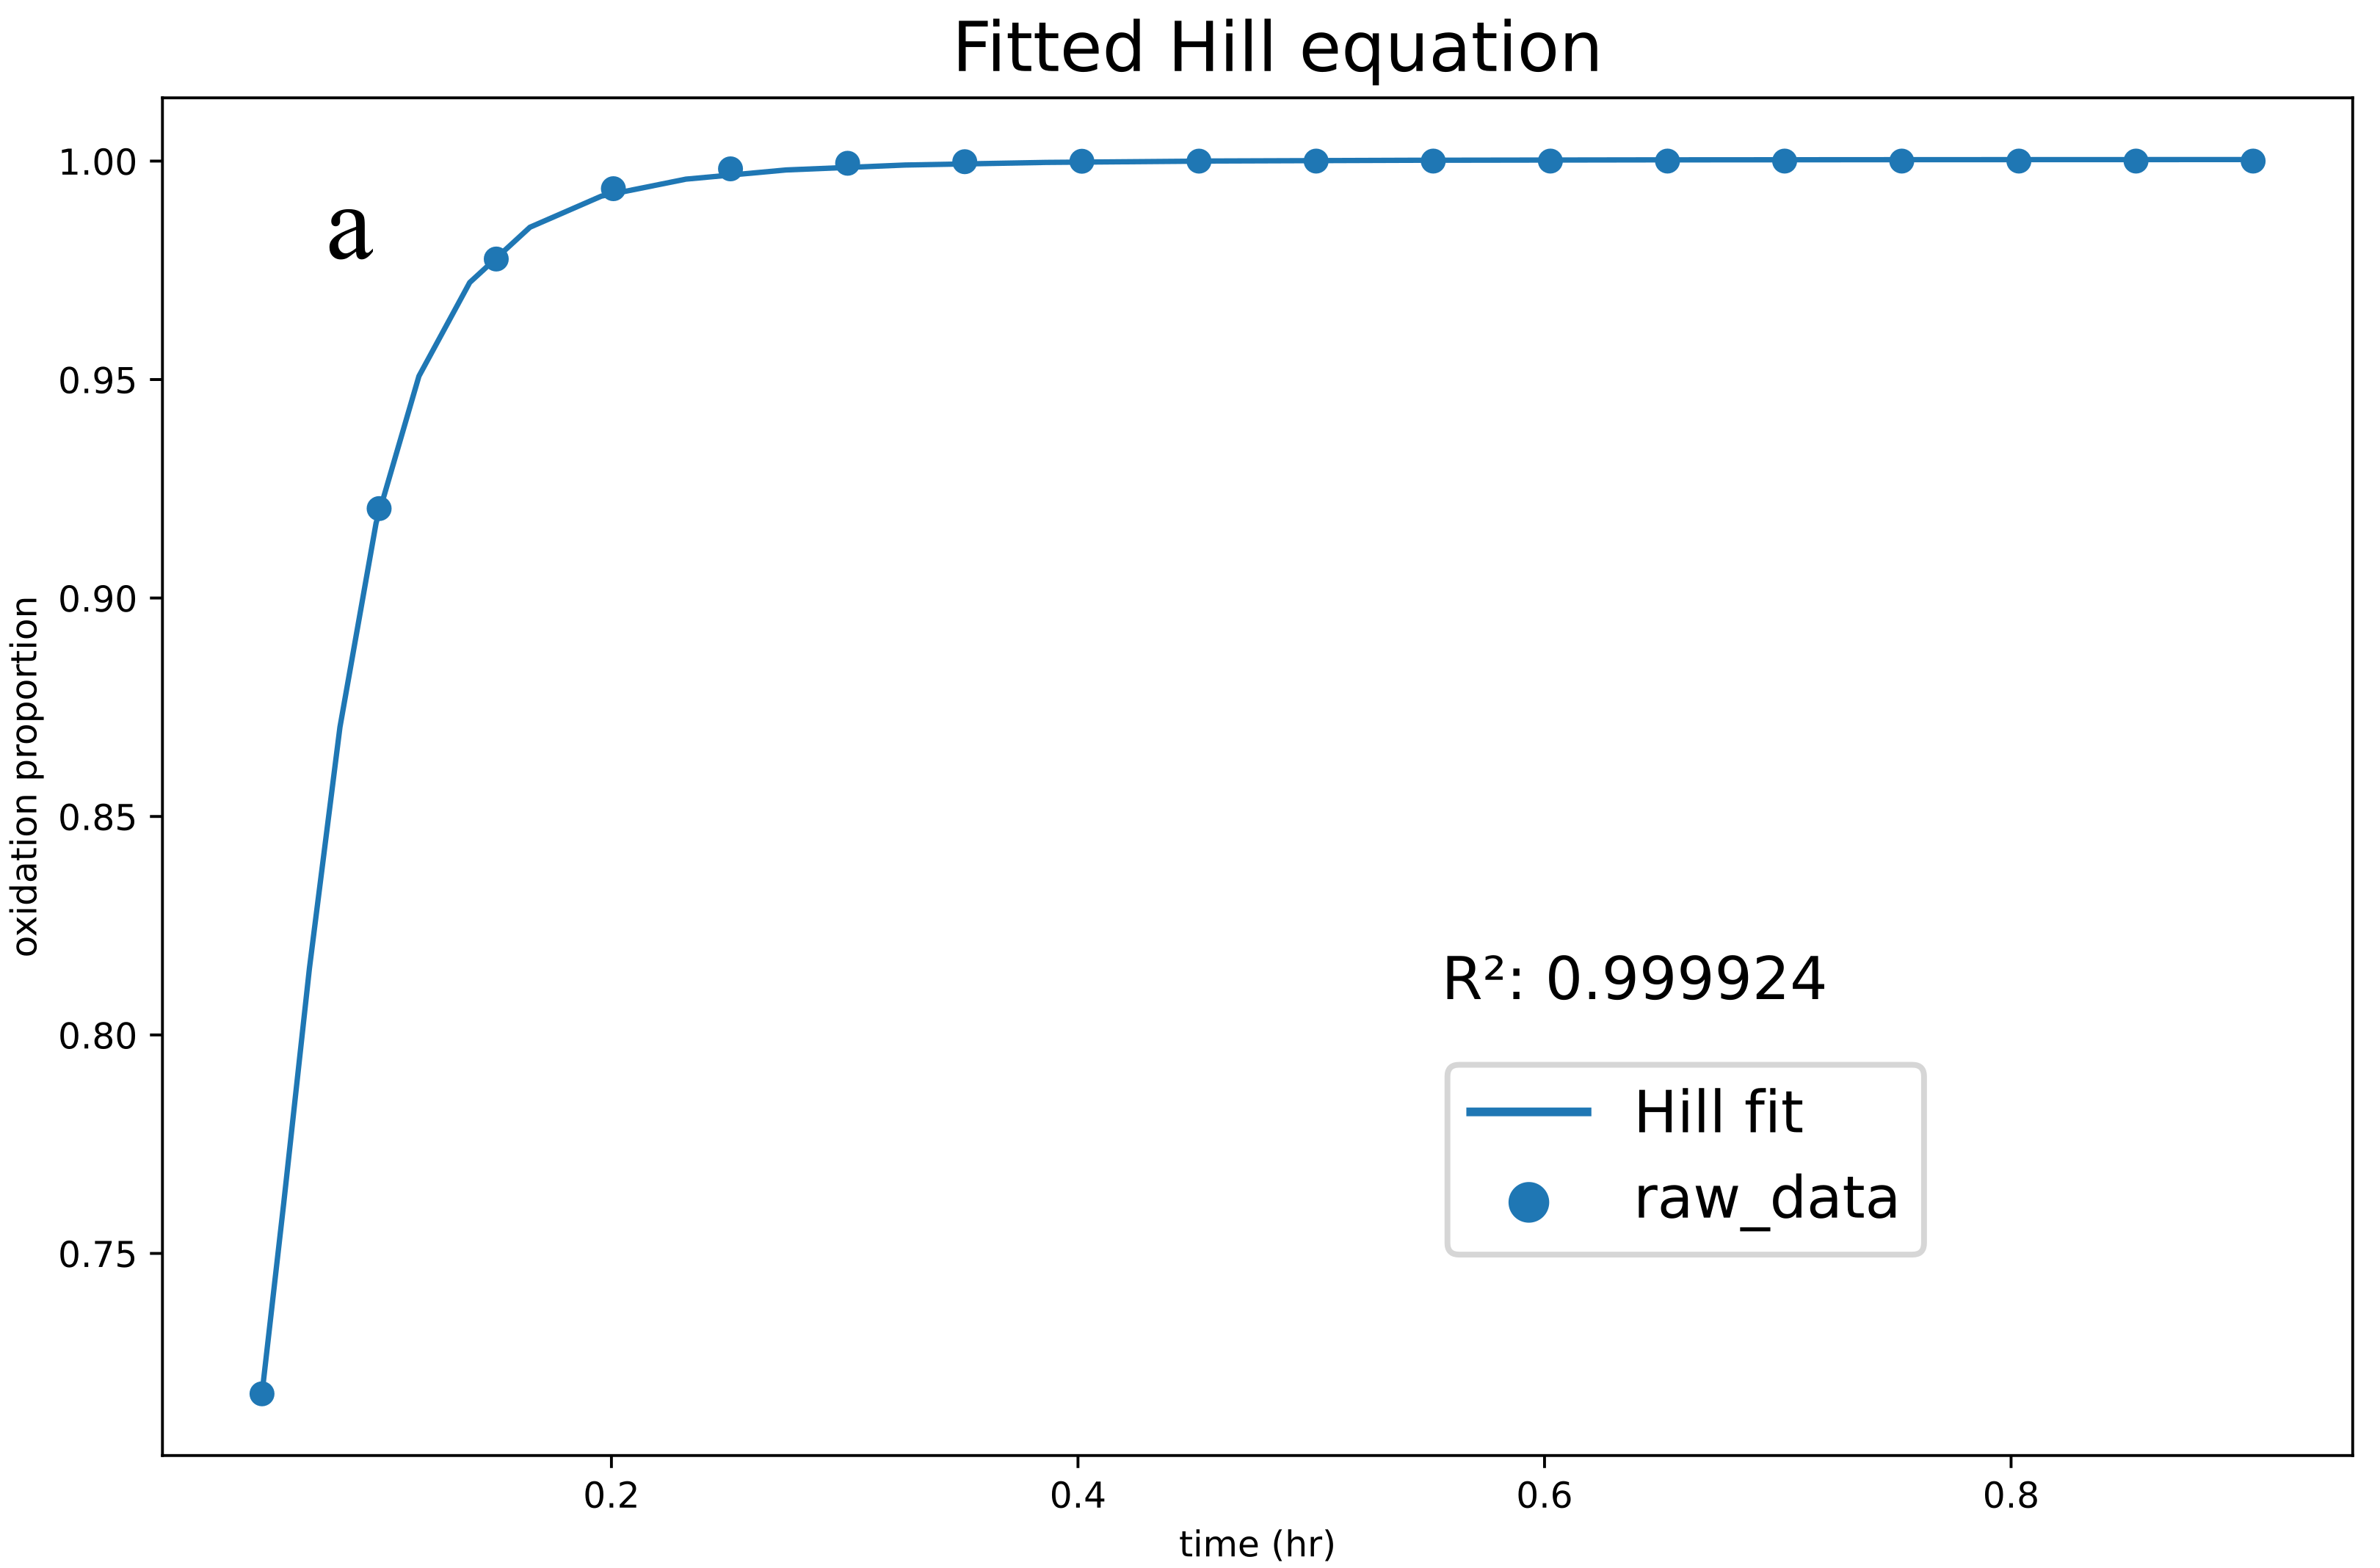
\includegraphics[width = 0.9\textwidth]{images/examples/20uM_regression.png}
    \vspace{5mm}
    \midrule
    \vspace{5mm}
    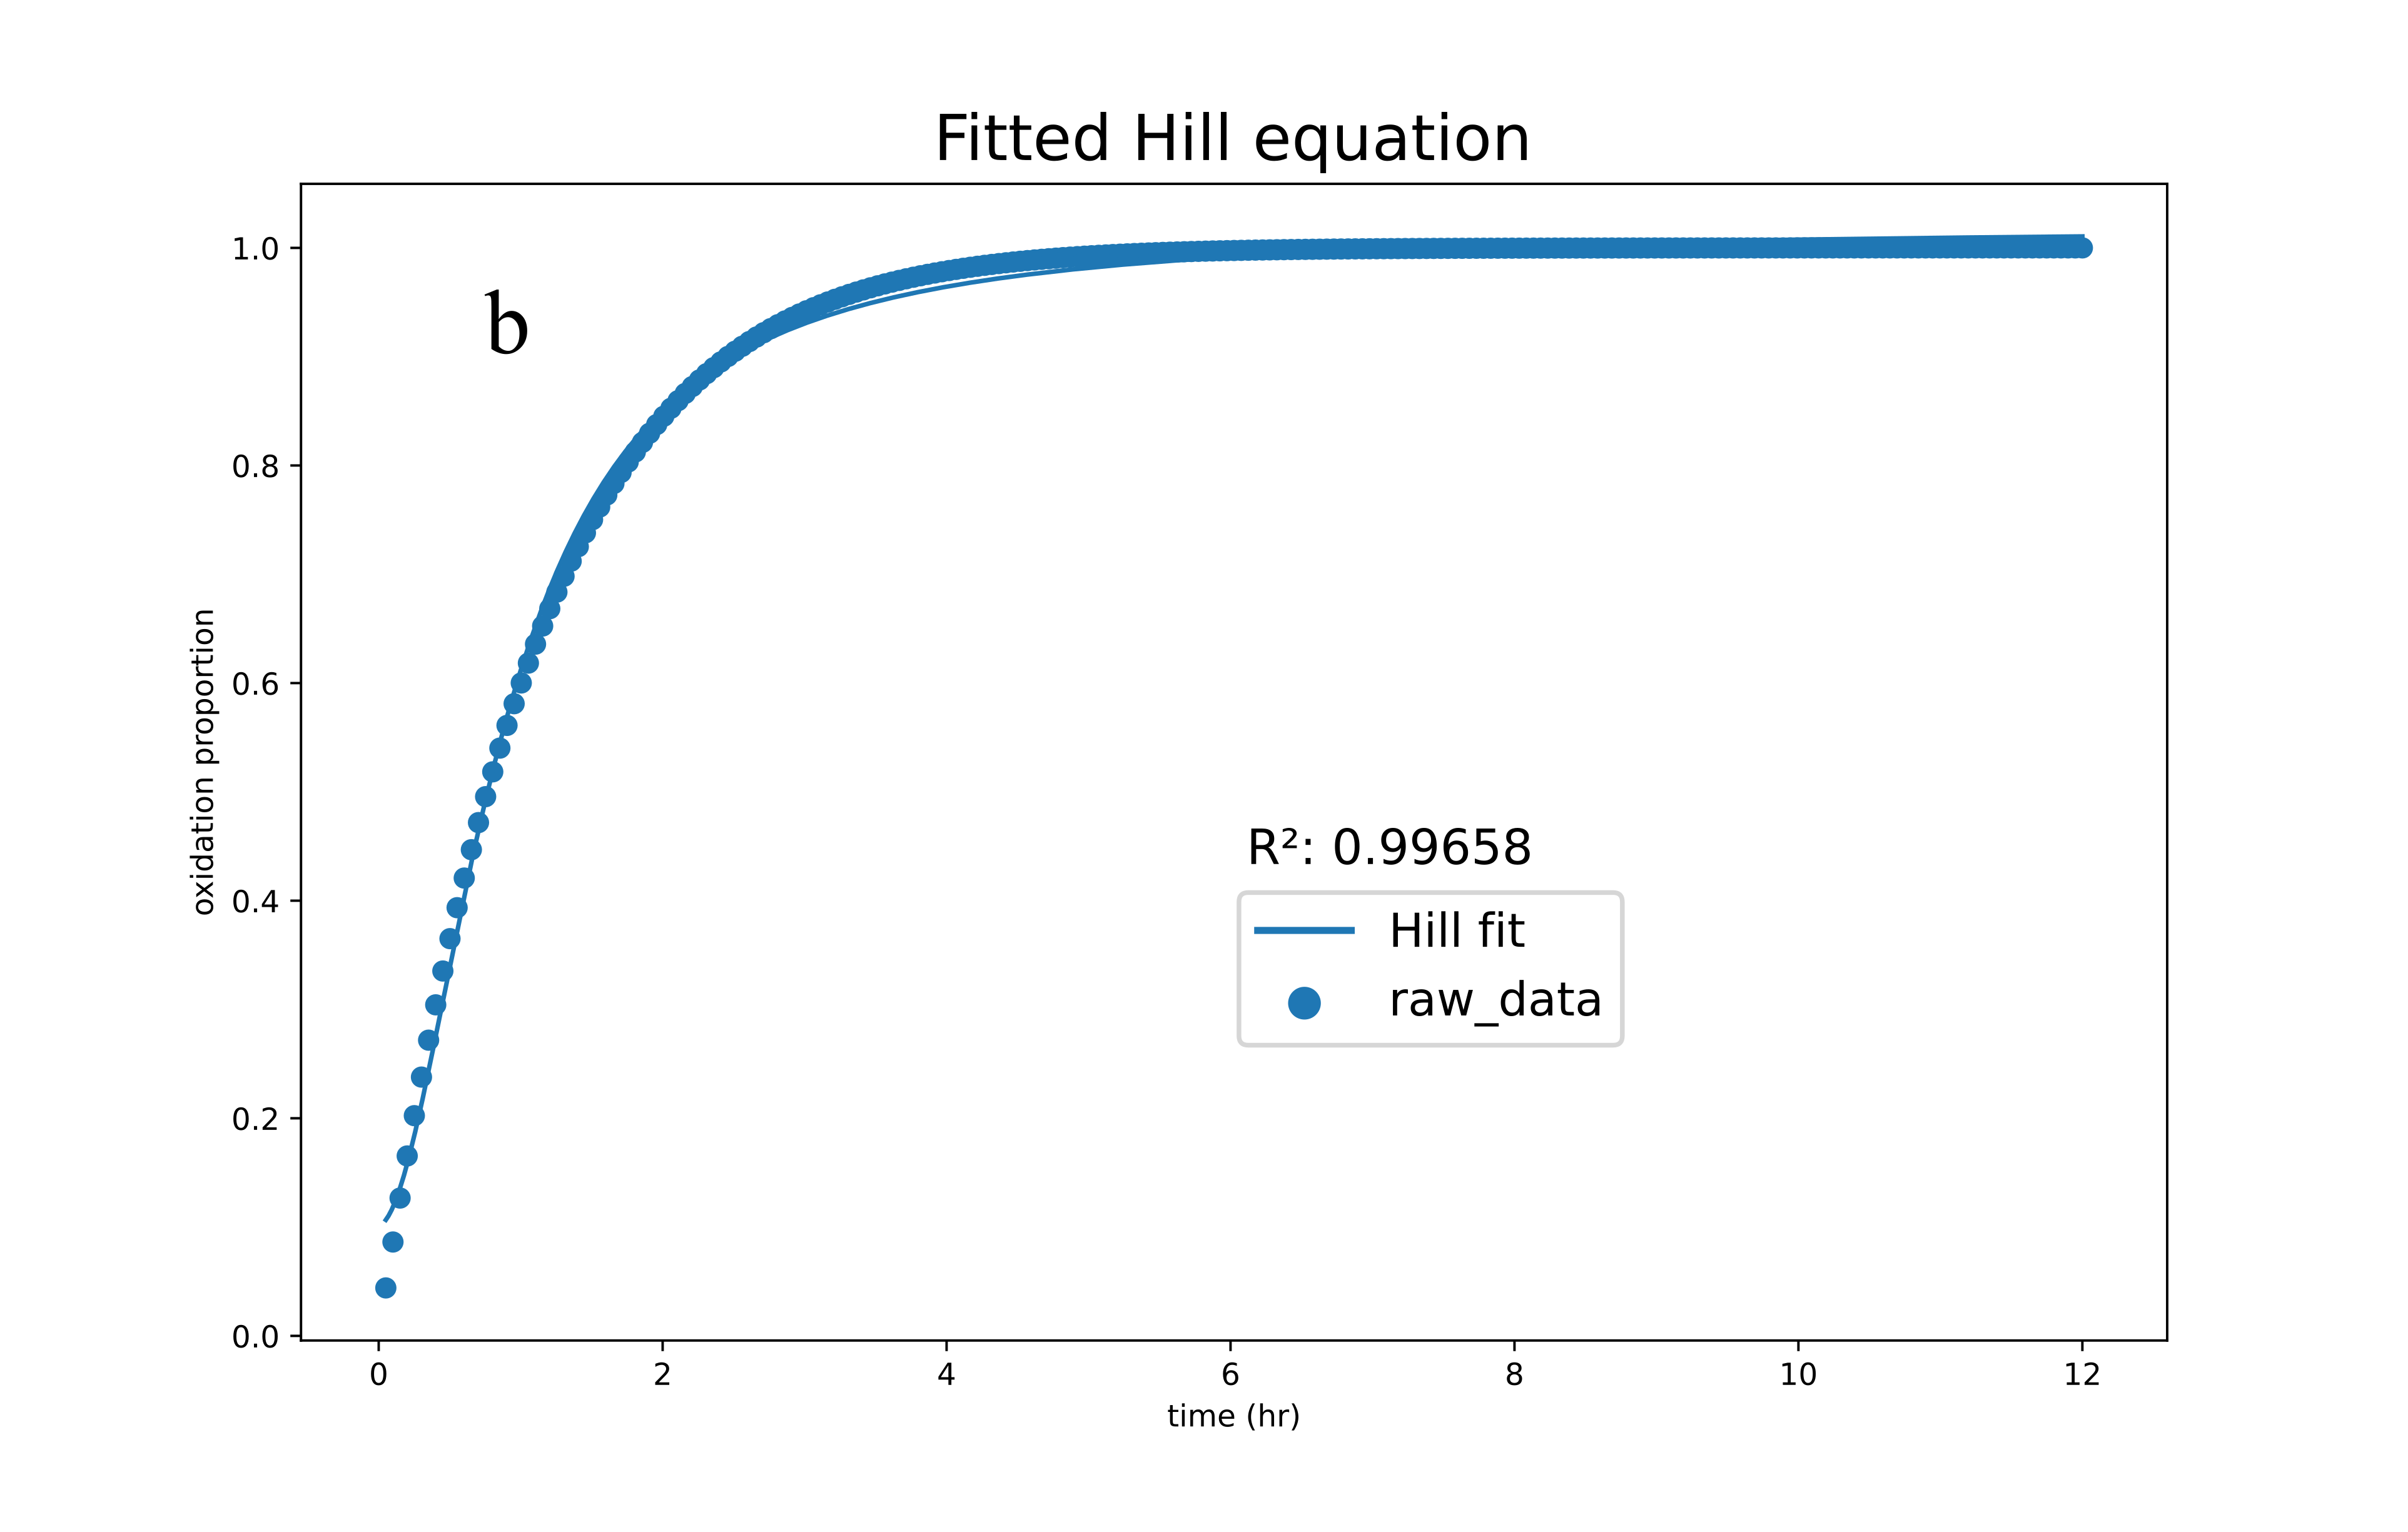
\includegraphics[width = 0.9\textwidth]{images/examples/10uM_biofilm_regression.png}
    \caption{
        The Hill-equation regressions for the oxidation plots of Figure \ref{beirao_et_al}, respectively. The high $R^2$ correlation supports that our chemical model of PDI recreates a sigmoidal biochemical relationship. The greater number of data points in panel b) is the consequence of a far longer simulation time than the simulation of panel a).
    }
    \label{hill_regression}
\end{figure}


\section{Sensitivity analyses}

\paragraph{Light intensity}
The sensitivity of simulation results to light intensities, across the range of $[10, 100,000] Lux$, was explored. The trend over this 4-log range, which is represented by Figure \ref{light_intensities}, is that the proportion of excited PS asymptotically approches 100\% and that minimal gains are observed beyond $\approx 13,000 lux$ from the perspective of exciting PSs. The influence of photobleaching appears to be negligible at the examined time length and light intensity, where a negative slope in the plotted excitation proportion over time would be indicative of photobleaching as a decreasing proportion of PSs are able to electronically excite.

\begin{figure}
    \centering
    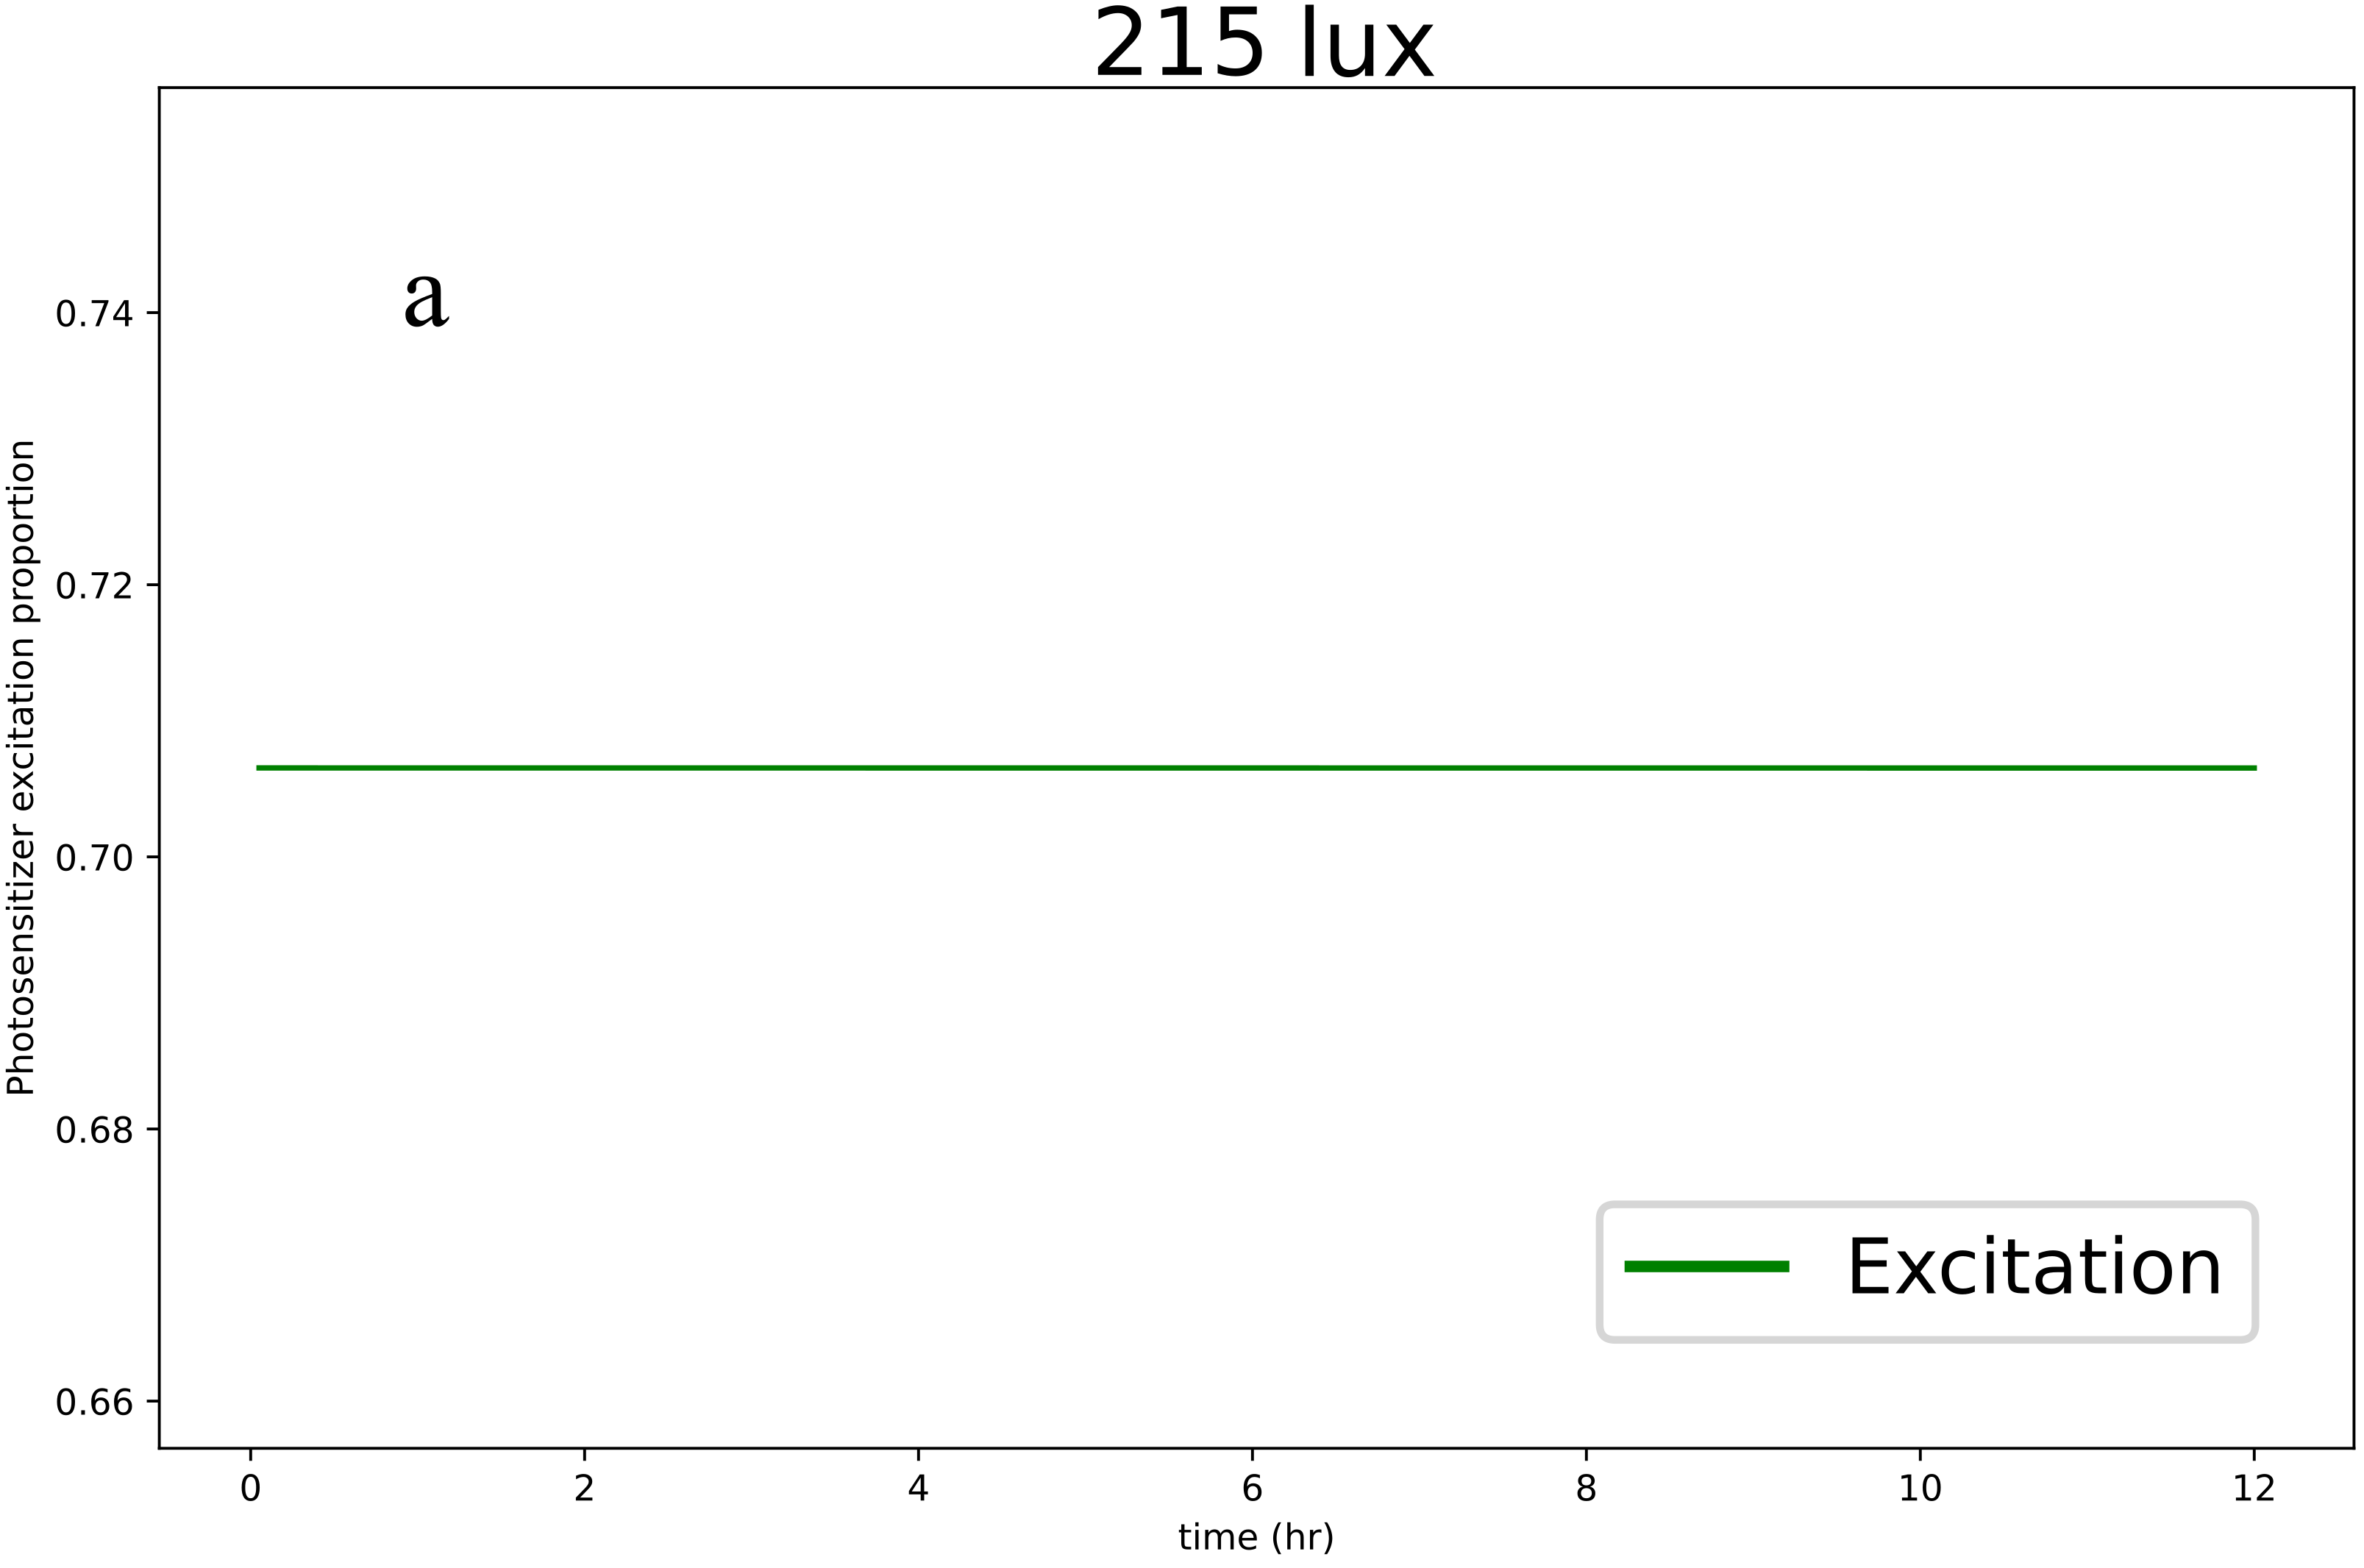
\includegraphics[width = 0.9\textwidth]{images/sensitivity_analyses/215_lux.png} \\
    \vspace{5mm}
    \midrule
    \vspace{5mm}
    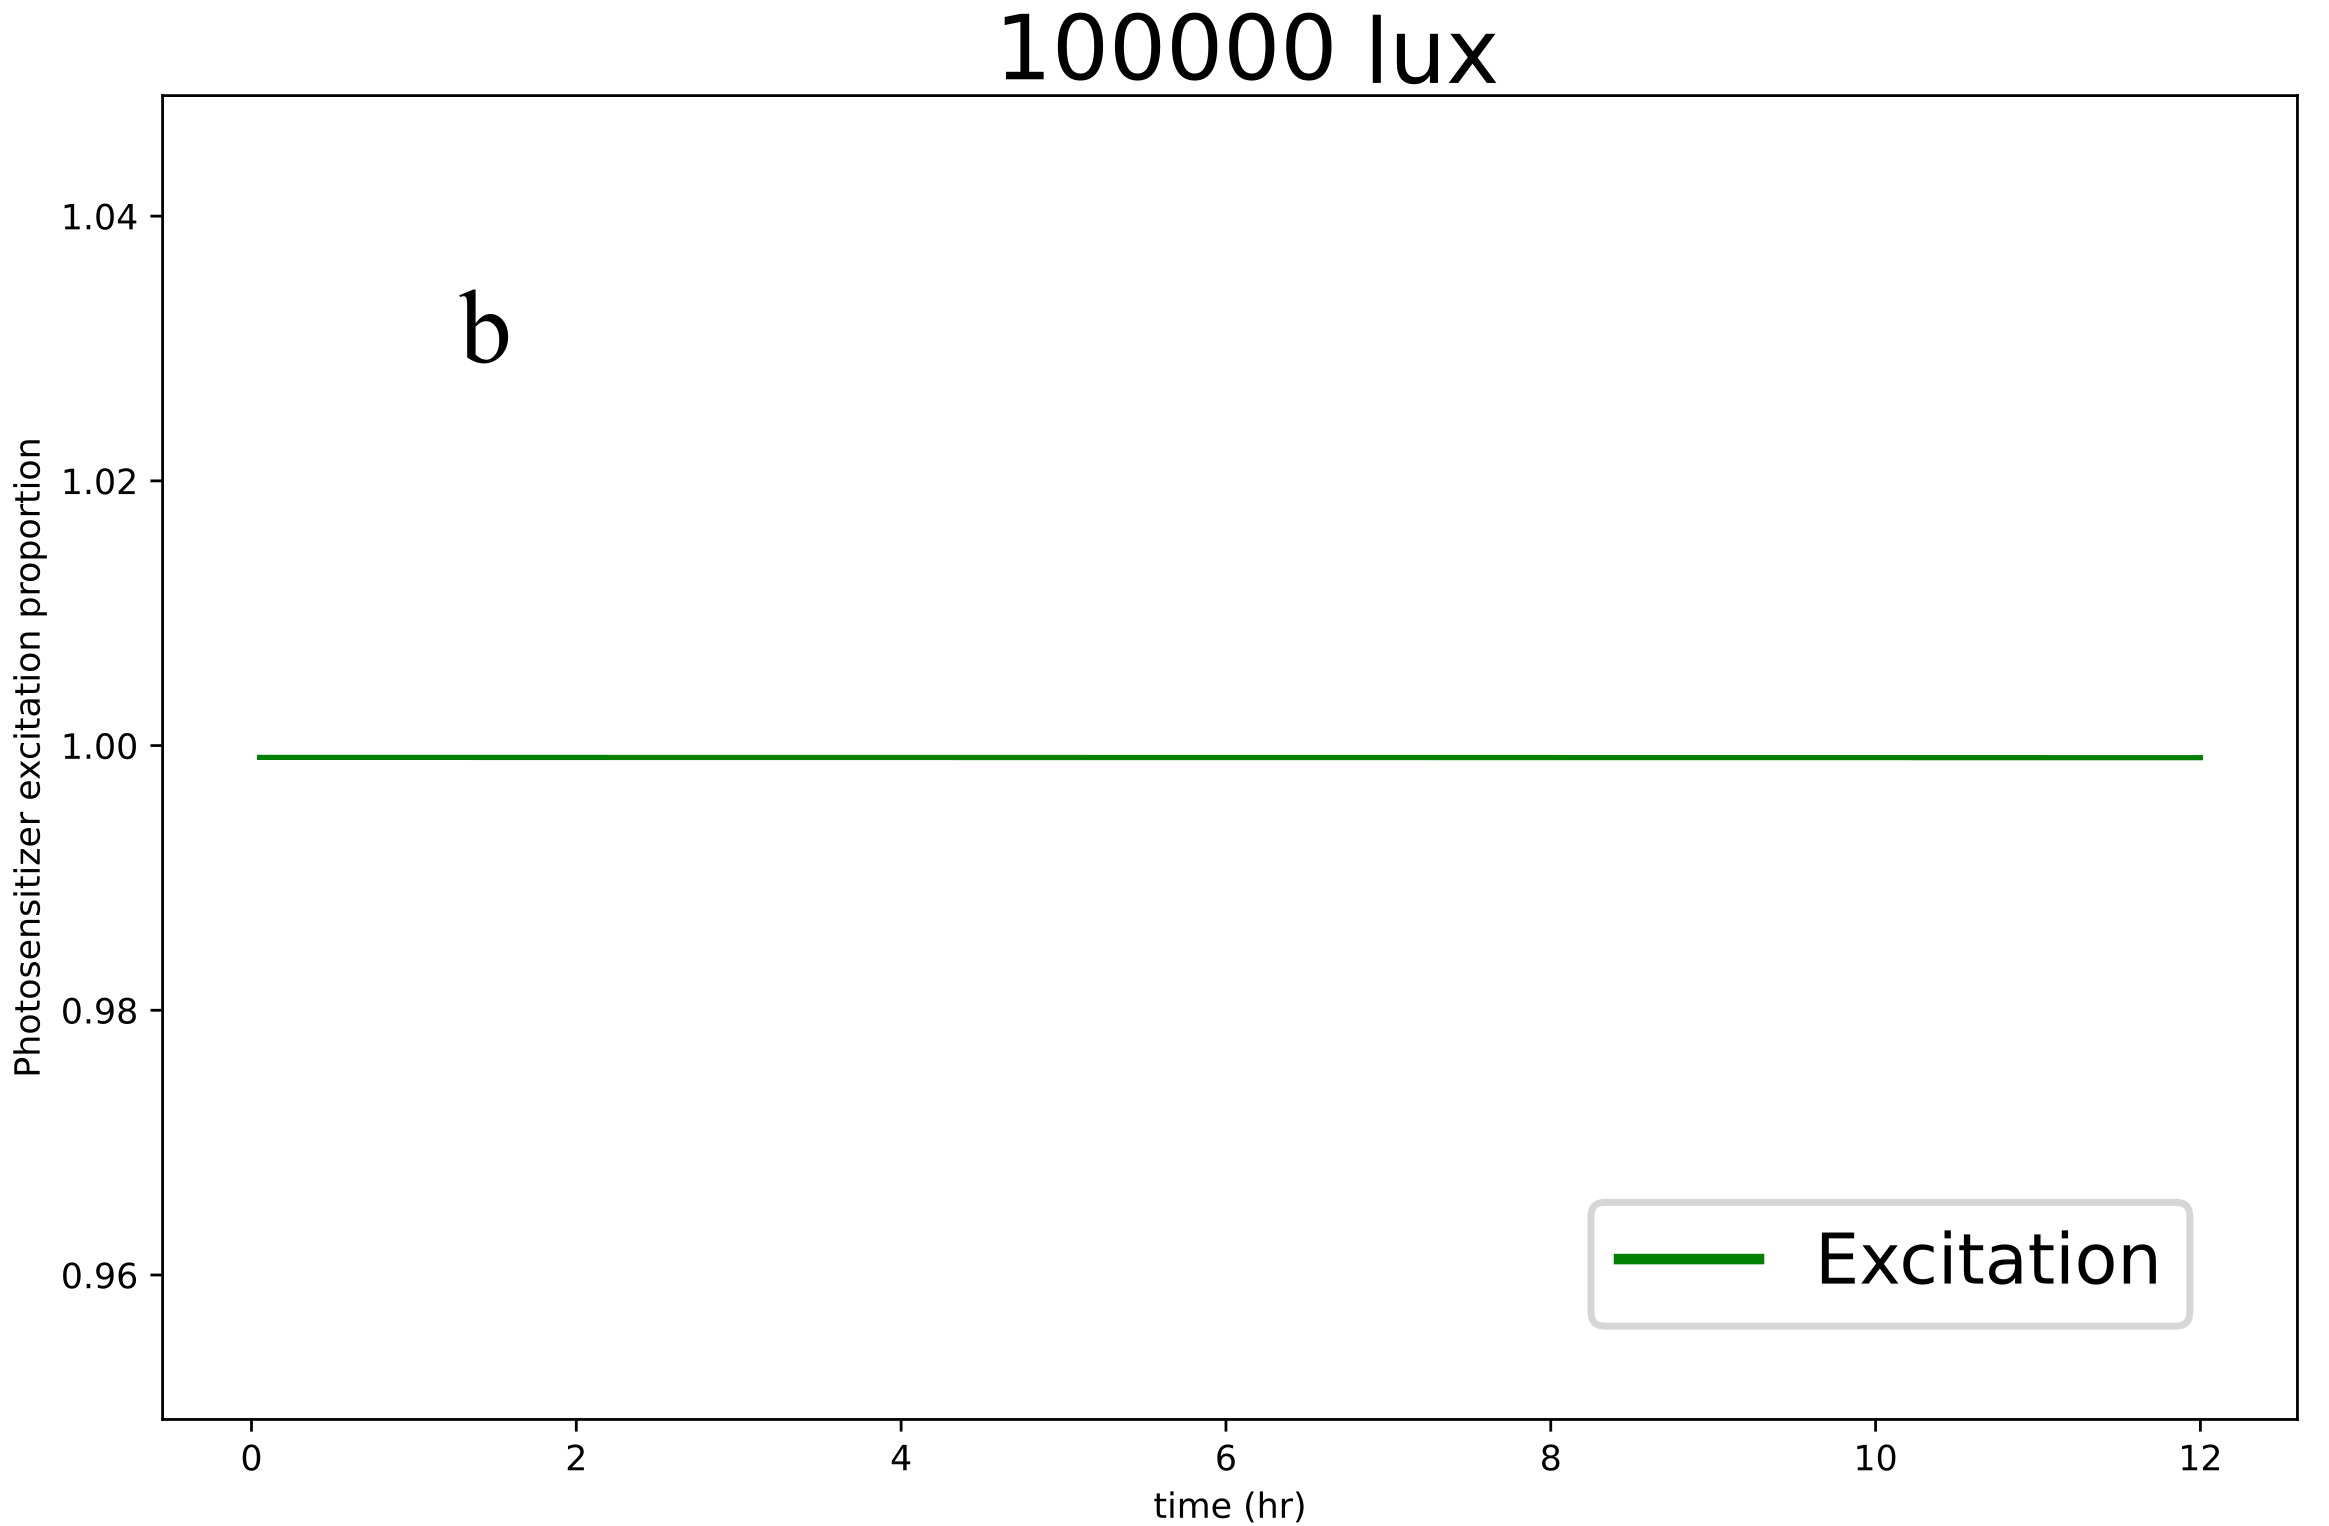
\includegraphics[width = 0.9\textwidth]{images/sensitivity_analyses/100000_lux.png}
    \caption{
        The proportion of excited PS at two contrasting light intensities: a) $215~Lux$ and b) $100000~Lux$. The subtle negative slope is the consequence of photobleaching, where the quantity of excitable PSs decreases over time. This effect is more prominent in b) than in a) since photobleaching is a function of light intensity.
    }
    \label{light_intensities}
\end{figure}

\section{Discussion}
The approximate alignment of inactivation between the PDIpy predictions and reported measurements by Beirao et al. supports that the underlying kinetic model represents essential PDI processes, however, the model has room for improvement. The predicted inactivations extensively varied, where simulations with low concentrations of PS reached the reported log-inactivation too late while simulations with high concentrations of PS reached the reported log-inactivation too early. This spread was interestingly relatively greater with the simulation of planktonic bacteria relative to the simulation of sessile bacteria, which suggests that readjusting the Hill parameters in Table \ref{hill_parameters} may resolve the discrepancy, since these parameter adjustments differ between the two simulation types. The discrepancy may alternatively be explained by greater experimental variability with planktonic bacteria than biofilm bacteria. Replicating other experimental studies will clarify the source and resolution of this discrepancy. 

The sensitivity analysis of light intensity revealed that the proportion of excited PSs plateaus beyond $\approx 10,000 lux$ as light intensity increases. This particular insight may be informative for experimentalists who are designing PDI systems with different light intensities, or who may want to separate observed light effects between $\ce{^1\Delta_g}$ generation from other effects of light per se. This type of broad inquiry over a 4-log value range furthermore exhibits the uniqueness of PDIpy relative to extant PDI models that neither embody the fundamental kinetics of PDI, which enable this kind of inquiry, nor provide an API interface that allows a user to efficiently execute numerous simulations with subtly different parameters.  

We believe that this kinetic model and its open-source implementation in PDIpy will practically support experimentalists in researching PDI technologies, and will ideally inspire other computational biologists to develop programs from this framework that can foster the discovery of new antibiotic methods and prevent antimicrobial resistant epedemics.

\section{Author Contributions}
\begin{description}
    \item[APF] Designed, executed, and codified the project.
    \item[JRK] Guidance and manuscript edits.
    \item[HLB] Guidance, manuscript edits, and funding.
\end{description}

\section{Acknowledgments}
The authors are grateful to Ethan Sean Chan for his development of the framework for iPDIpy, which will be introduced in a future release of PDIpy. The authors thank the members of the Buckley and Wolff Groups at the University of Victoria for contributing ideas and data that were used to refine this PDI model. Andrew finally thanks Hiroaki Imoto for his contributions and guidance in developing the HillFit module that was used to fit data in PDIpy.